% Enriched Lawvere Theories for Operational Semantics
% John C. Baez and Christan Williams
% 2018/10/31

\documentclass{amsart}
\usepackage{geometry}
\usepackage{amsmath}
\usepackage{amssymb}
\usepackage{bussproofs}
\usepackage[utf8]{inputenc}
\usepackage[english]{babel}
\usepackage{amsthm}
\usepackage{mathtools}
\usepackage{authblk}
\usepackage{pict2e}
\usepackage[mathscr]{euscript}

\usepackage{tikz}
\usetikzlibrary{matrix}

%drawing
\usepackage{tikz-cd}
\usepackage{tikzit}
\documentclass{beamer}
\usetheme{Goettingen}
\usecolortheme{wolverine}
%\usefonttheme{serif}

\usepackage{geometry}
\usepackage{amsmath}
\usepackage{amssymb}
\usepackage{bussproofs}
\usepackage[utf8]{inputenc}
\usepackage[english]{babel}
\usepackage{amsthm}
\usepackage{mathtools}
%\usepackage{authblk}
\usepackage{pict2e}
\usepackage[mathscr]{euscript}
\usepackage{tikz-cd}
\tikzstyle{none}=[inner sep=0pt]
\tikzstyle{circ}=[circle,fill=black,draw,inner sep=3pt]
\usepackage{fancybox}
\usepackage[all,2cell]{xy} \UseAllTwocells
\usetikzlibrary{arrows, positioning, intersections}
\input{coya-tikz.tex}
\tikzset{%
	symbol/.style={%
		draw=none,
		every to/.append style={%
			edge node={node [sloped, allow upside down, auto=false]{$#1$}}}
	}
}

% hyperlinks
% \usepackage{color}
% \definecolor{myurlcolor}{rgb}{0.5,0,0}
% \definecolor{mycitecolor}{rgb}{0,0,1}
% \definecolor{myrefcolor}{rgb}{0,0,1}
% \usepackage[pagebackref]{hyperref}
% \hypersetup{colorlinks,
% linkcolor=myrefcolor,
% citecolor=mycitecolor,
% urlcolor=myurlcolor}

% \newcommand{\define}[1]{{\bf \boldmath{#1}}}
% \renewcommand*{\backref}[1]{(Referred to on page #1.)}

% theorems

% \theoremstyle{definition}
% \newtheorem{theorem}{Theorem}
% \newtheorem{definition}[theorem]{Definition}
% \newtheorem{lemma}[theorem]{Lemma}
% \newtheorem{example}[theorem]{Example}
% \newtheorem{corollary}{Corollary}[theorem]

\def\rd{\rotatebox[origin=c]{90}{$\dashv$}} %rotate dash right
\def\ld{\rotatebox[origin=c]{-90}{$\dashv$}} %rotate dash left

% categories

\newcommand{\Th}{\mathsf{Th}}
\newcommand{\Gph}{\mathsf{Gph}}
\newcommand{\Set}{\mathsf{Set}}
\newcommand{\Grp}{\mathsf{Grp}}
\newcommand{\Cat}{\mathsf{Cat}}
\newcommand{\Law}{\mathsf{Law}}
\newcommand{\Mnd}{\mathrm{Mnd}}
\newcommand{\Top}{\mathsf{Top}}
\newcommand{\Mon}{\mathsf{Mon}}
\newcommand{\Alg}{\mathsf{Alg}}
\newcommand{\CCC}{\mathsf{CCC}}
\newcommand{\Pos}{\mathsf{Pos}}
\newcommand{\Mod}{\mathsf{Mod}}
\newcommand{\FinSet}{\mathsf{FinSet}}
\newcommand{\NN}{\mathsf{N}}
\newcommand{\A}{\mathsf{A}}
\newcommand{\V}{\mathsf{V}}
\newcommand{\W}{\mathsf{W}}
\newcommand{\D}{\mathsf{D}}
\newcommand{\C}{\mathsf{C}}
\newcommand{\R}{\mathsf{R}}
\newcommand{\X}{\mathsf{X}}
\newcommand{\K}{\mathsf{K}}
\newcommand{\J}{\mathsf{J}}
\newcommand{\T}{\mathsf{T}}
\newcommand{\Kl}{\mathsf{Kl}}
\newcommand{\LTS}{\mathsf{LTS}}

\newcommand{\FC}{\mathrm{FC}}
\newcommand{\FP}{\mathrm{FP}}
\newcommand{\FS}{\mathrm{FS}}
\newcommand{\UC}{\mathrm{UC}}
\newcommand{\UP}{\mathrm{UP}}
\newcommand{\UG}{\mathrm{UG}}

\newcommand{\op}{\mathrm{op}}
\newcommand{\Obj}{\mathrm{Ob}}

\newcommand{\pic}{$\pi$-calculus}

\newcommand{\pfk}{\pitchfork}
\newcommand{\maps}{\colon}
\newcommand{\id}{\mathrm{id}}

\newcommand{\ul}[1]{\underline{#1}}


\title{Enriched Lawvere Theories\\ for Operational Semantics}
\author{John C. Baez: baez@math.ucr.edu\\ Christian Williams: williams@same}
\institute{University of California, Riverside}
\date{SYCO 4, May 22 2019}

\begin{document}
\frame{\titlepage}

\begin{frame}{Introduction}
  How do we integrate syntax and semantics?
  \[\begin{array}{ll}
      \text{type} & \text{object}\\
      \text{term} & \text{morphism}\\
      \text{rewrite} & \text{2-morphism}\\
    \end{array}\]
  \[\begin{tikzcd}[ampersand replacement=\&]
      (\lambda x.x+x \; \; 2) \ar{r}{\beta} \& 2+2 \ar{r}{+} \& 4
    \end{tikzcd}\]
\end{frame}
\begin{frame}{Change of semantics}
  \[\begin{tikzcd}[column sep=small, ampersand replacement=\&]
\Gph \arrow[bend left,below]{rr}{\FC}
\& \ld \&
\arrow[bend left,above]{ll}{\UG} \Cat \arrow[bend left,below]{rr}{\FP}
\& \ld \&
\arrow[bend left,above]{ll}{\UC} \Pos \arrow[bend left,below]{rr}{\FS}
\& \ld \&
\Set \arrow[bend left,above]{ll}{\UP}
\end{tikzcd}\]

\[\begin{array}{ll}
    \FC_* & \text{maps small-step to big-step operational semantics.}\\
    \FP_* & \text{maps big-step to full-step operational semantics.}\\
    \FS_* & \text{maps full-step to denotational semantics.}\\
\end{array}\]

\end{frame}

\section{theories}
\subsection{Lawvere theories}
\begin{frame}{Lawvere theories}
  A \textbf{Lawvere theory} is a category $\T$ whose objects are finite powers of a distinguished object $t = \tau(1)$.
  $$\tau\maps \mathbb{N}^{\op}\to \T$$
  Morphisms $t^n\to t$ are $n$-ary operations, and commuting diagrams are equations.\\~\\
  Classical algebra is represented and internalized in any category with finite products.
\end{frame}
\begin{frame}{Models}
  Let $\C$ be a category with finite products.\\~\\
  A \textbf{model} of a Lawvere theory $\T$ in $\C$ is a product-preserving functor $\mu\maps \T\to \C$. A morphism of models is a natural transformation. \\~\\
  These form a category $\Mod(\T,\C)$. For example, $\Mod(\Th(\Grp),\Top)$ is the category of topological groups.
\end{frame}
\subsection{theories and monads}
\begin{frame}{Monadicity}
  Another way to describe algebraic structure is by \textit{monads}. Theories induce ``free-forgetful'' adjunctions: 
  \[\begin{tikzcd}[column sep=small, ampersand replacement=\&]
      \Set \arrow[bend left,below]{rr}{F}
      \& {\phantom{AA} \ld} \&
      \arrow[bend left,above]{ll}{U} \Mod(\T,\Set).
    \end{tikzcd}\]
  \[\begin{array}{lll}
      U :: \mu\mapsto \mu(1) && F :: n\mapsto \T(n,-)\\
      && \text{extends to $\Set$ by colimit.}
    \end{array}\]\\
  This induces a monad $T$ on $\Set$, and we have that:
  $$T\text{-Alg} \simeq \Mod(\T,\Set).$$
\end{frame}

\section{enrichment}
\subsection{enriched categories}
\begin{frame}{Enriched categories}
Let $\V$ be a monoidal category. A \textbf{$\V$-enriched category} is:
  \[\begin{array}{ll}
\text{object set} & \Obj(\C)\\
\text{hom function} & \C(-,-)\maps \Obj(\C) \times \Obj(\C) \to \Obj(\V)\\
\text{composition} & \circ_{a,b,c}\maps\C(b,c) \times \C(a,b) \to \C(a,c)\\
\text{identity} & i_a\maps 1_\V \to\C(a,a)\\
    \end{array}\]
  with composition associative and unital.\\
  A \textbf{$\V$-functor} $F\maps \C\to \D$ is:
  \[\begin{array}{ll}
\text{object function} & F\maps \Obj(\C) \to \Obj(\D)\\
\text{hom morphisms} & F_{ab}\maps \C(a,b) \to \D(F(a),F(b))\\
    \end{array}\]
  preserving composition and identity.\\
  A \textbf{$\V$-natural transformation} $\alpha\maps F \Rightarrow G$ is:
\[\begin{array}{ll}
\text{components} & \alpha_a \maps 1_\V \to \D(F(a),G(a))\\
\end{array}\]
 which is ``natural'' in $a$. These form the 2-category \textbf{$\V\Cat$}. 
\end{frame}
\subsection{enriched limits}
\begin{frame}{Enriched limits}
  a
\end{frame}
\begin{frame}{Preservation}
  a
\end{frame}

\section{enriched theories}
\subsection{enriched Lawvere theories}
\begin{frame}{Enriched Lawvere theories}
  a
\end{frame}
\begin{frame}{Generalized arities}
  a
\end{frame}
\subsection{enriched monadicity}
\begin{frame}{Enriched monadicity}
  a
\end{frame}
\subsection{examples}
\begin{frame}{Example: pseudomonoid}
  \[ \Th(\mathrm{PsMon}) \]
  \[\begin{array}{lll}
  \textbf{type}\\ M & \text{pseudomonoid}\\ \\
  \textbf{operations}\\ m\maps M^2 \to M & \text{multiplication}\\
                e\maps1 \to M & \text{identity}\\ \\
  \textbf{rewrites}\\ \alpha \colon m(m \times \id_M) \cong m (\id_M \times m) & \text{associator}\\
                \lambda\maps  m(e \times \id_M) \cong \id_M & \text{left unitor}\\
                \rho\maps m(\id_M \times e) \cong \id_M & \text{right unitor}\\ \\
  \textbf{equations} & \text{pentagon, triangle}
  \end{array}\]
\end{frame}
\begin{frame}{Example: cartesian object}
  
  \[ \Th(\mathsf{Cart}) \]
  \[\begin{array}{lllllll}
      \textbf{type}\\ \X & \text{cartesian object}\\ \\
      \textbf{operations}\\ m \maps \X^2 \to \X & \text{product} \\ 
        e \maps 1 \to \X & \text{terminal element} \\ \\
      \textbf{rewrites}\\
      \bigtriangleup\maps \mathrm{id}_\X \Longrightarrow m \circ\, \Delta_\X & \text{unit of $m \vdash \Delta_\X$}\\
      \pi\maps \Delta_\X \circ m \Longrightarrow \mathrm{id}_{\X^2} & \text{counit of $m \vdash \Delta_\X$}\\
      \top\maps \mathrm{id}_\X \Longrightarrow e \,\circ\, !_\X & \text{unit of $e \vdash !_\X$} \\
      \epsilon \maps !_\X \, \circ \, e \Longrightarrow \mathrm{id}_{1} & \text{counit of $e \vdash !_\X$} \\\\
 \textbf{equations}  & \text{triangle identities}
 \end{array}\]
\end{frame}

\section{natural number arities}
\subsection{arity subcategory}
\begin{frame}{Natural numbers in $\mathsf{V}$}
  a
\end{frame}
\subsection{equivalences}
\begin{frame}{Equivalences}
  a
\end{frame}

\section{change of semantics}
\subsection{change of base}
\begin{frame}{Change of base}
  a
\end{frame}
\subsection{preserving theories}
\begin{frame}{Preservation of theories}
  a
\end{frame}

% \section{grothendieck?}
% \subsection{category of all theories}
% \begin{frame}
  
% \end{frame}

\section{applications}
\subsection{combinators}
\begin{frame}{The $\mathsf{SKI}$-combinator calculus}
  a
\end{frame}
%\subsection{theory}
\begin{frame}{The theory of $\mathsf{SKI}$}
  a
\end{frame}
\subsection{change of base}
\begin{frame}{Change of semantics}
  a
\end{frame}
% \subsection{change of theory}
% \begin{frame}{Change of theory}
%   a
% \end{frame}
% \subsection{bisimulation}
\begin{frame}{Bisimulation}
  a
\end{frame}

\begin{frame}{Conclusion}

\end{frame}

\end{document}
\tikzstyle{none}=[inner sep=0pt]
\tikzstyle{circ}=[circle,fill=black,draw,inner sep=3pt]
\usepackage{fancybox}
\usepackage[all,2cell]{xy} \UseAllTwocells
\usetikzlibrary{arrows, positioning, intersections}
\newcommand{\mult}[1]
{
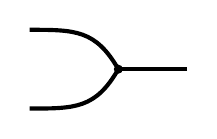
\begin{tikzpicture}
\scalebox{1}{
		\node [style=none] (0) at (1, -0) {};
		\node  [circle,draw,inner sep=1pt,fill]   (1) at (0.125, -0) {};
		\node [style=none] (2) at (-1, 0.5) {};
		\node [style=none] (3) at (-1, -0.5) {};
		\draw[line width = 1.5pt] (0.center) to (1.center);
		\draw[line width = 1.5pt] [in=0, out=120, looseness=1.20] (1.center) to (2.center);
		\draw[line width = 1.5pt] [in=0, out=-120, looseness=1.20] (1.center) to (3.center);
}
      \end{tikzpicture}
}

\newcommand{\unit}[1]
{
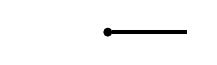
\begin{tikzpicture}
\scalebox{1}{
		\node [style=none] (0) at (1, -0) {};
		\node [style=none] (1) at (-1, -0) {};
		\node  [circle,draw,inner sep=1pt,fill]   (2) at (0, -0) {};
		\draw[line width = 1.5pt] (0.center) to (2);
}
      \end{tikzpicture}
}

\newcommand{\unitl}[1]
{
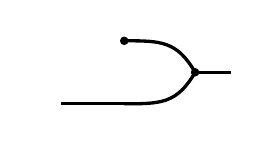
\begin{tikzpicture}
\scalebox{0.8}{
		\node [style=none] (0) at (0.7, -0) {};
		\node  [circle,draw,inner sep=1.2pt,fill]   (1) at (0.125, -0) {};
		\node  [circle,draw,inner sep=1.2pt,fill]   (2) at (-1, 0.5) {};
		\node [style=none] (3) at (-1, -0.5) {};
		\node [style=none] (4) at (-2, -0.5) {};
		\draw [line width = 1.5pt] (0.center) to (1.center);
		\draw [in=0, out=120, looseness=1.20, line width = 1.5pt] (1.center) to (2.center);
		\draw [in=0, out=-120, looseness=1.20, line width = 1.5pt] (1.center) to (3.center);
		\draw [line width = 1.5pt] (4.center) to (3.center);
}
\end{tikzpicture}
}

\newcommand{\unitr}[1]
{
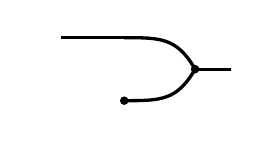
\begin{tikzpicture}
\scalebox{0.8}{
		\node [style=none] (0) at (0.7, -0) {};
		\node  [circle,draw,inner sep=1.2pt,fill]   (1) at (0.125, -0) {};
		\node  [circle,draw,inner sep=1.2pt,fill]   (2) at (-1, -0.5) {};
		\node [style=none] (3) at (-1, 0.5) {};
		\node [style=none] (4) at (-2, 0.5) {};
		\draw [line width = 1.5pt] (0.center) to (1.center);
		\draw [in=0, out=120, looseness=1.20, line width = 1.5pt] (1.center) to (3.center);
		\draw [in=0, out=-120, looseness=1.20, line width = 1.5pt] (1.center) to (2.center);
		\draw [line width = 1.5pt] (4.center) to (3.center);
}
\end{tikzpicture}
}

\newcommand{\idone}[1]
{
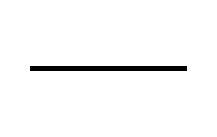
\begin{tikzpicture}
\scalebox{1}{
		\node [style=none] (0) at (-1, -0) {};
		\node [style=none] (1) at (1, -0) {};
		\node [style=none] (2) at (0, 0.5) {};
		\node [style=none] (3) at (0, -0.5) {};
		\draw[line width = 1.5pt] (1.center) to (0.center);
}
\end{tikzpicture} 
}


\newcommand{\assocl}[1]
{
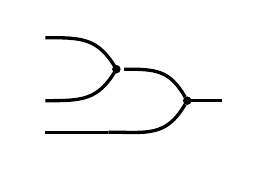
\begin{tikzpicture}
\scalebox{0.8}{
		\node  [circle,draw,inner sep=1.2pt,fill]   (0) at (0.125, -0) {};
		\node [style=none] (1) at (-1, 0.5) {};
		\node [style=none] (2) at (-1, -0.5) {};
		\node [style=none] (3) at (0, -1) {};
		\node [style=none] (4) at (1.8, -0.5) {};
		\node [style=none] (5) at (0.25, -0) {};
		\node  [circle,draw,inner sep=1.2pt,fill]   (6) at (1.25, -0.5) {};
		\node [style=none] (7) at (-1, -1) {};
		\draw [in=0, out=120, looseness=1.20, line width = 1.5pt] (0.center) to (1.center);
		\draw [in=0, out=-120, looseness=1.20, line width = 1.5pt] (0.center) to (2.center);
		\draw [line width = 1.5pt] (4.center) to (6);
		\draw [in=0, out=120, looseness=1.20, line width = 1.5pt] (6) to (5.center);
		\draw [in=0, out=-120, looseness=1.20, line width = 1.5pt] (6) to (3.center);
		\draw [line width = 1.5pt] (3.center) to (7.center);
}
      \end{tikzpicture}
}


\newcommand{\assocr}[1]
{
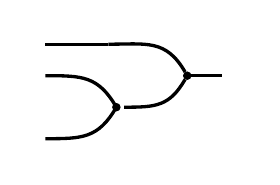
\begin{tikzpicture}
\scalebox{.8}{
		\node  [circle,draw,inner sep=1.2pt, fill]   (0) at (0.125, -0.5) {};
		\node [style=none] (1) at (-1, -1) {};
		\node [style=none] (2) at (-1, 0) {};
		\node [style=none] (3) at (0, 0.5) {};
		\node [style=none] (4) at (1.8, 0) {};
		\node [style=none] (5) at (0.25, -0.5) {};
		\node  [circle,draw,inner sep=1.2pt, fill]   (6) at (1.25, 0) {};
		\node [style=none] (7) at (-1, 0.5) {};
		\draw [in=0, out=-120, looseness=1.20, line width = 1.5pt] (0.center) to (1.center);
		\draw [in=0, out=120, looseness=1.20, line width = 1.5pt] (0.center) to (2.center);
		\draw [line width = 1.5pt] (4.center) to (6);
		\draw [in=0, out=-120, looseness=1.20, line width = 1.5pt] (6) to (5.center);
		\draw [in=0, out=120, looseness=1.20, line width = 1.5pt] (6) to (3.center);
		\draw [line width = 1.5pt] (3.center) to (7.center);
}
      \end{tikzpicture}
    }

\newcommand{\leftmost} {
\begin{tikzpicture}
	\begin{pgfonlayer}{nodelayer}
		\node [style=none] (0) at (0.5, 8) {};
		\node [style=none] (1) at (0.5, 7) {};
		\node [circle,draw,inner sep=1.2pt, fill] (2) at (1.5, 7.5) {};
		\node [style=none] (3) at (1.5, 6.5) {};
		\node [style=none] (4) at (0.5, 6.5) {};
		\node [style=none] (5) at (2.5, 7) {};
		\node [style=none] (6) at (2.5, 6) {};
		\node [style=none] (7) at (0.5, 6) {};
		\node [style=none] (8) at (3.5, 6.5) {};
		\node [style=none] (9) at (4, 6.5) {};
	\end{pgfonlayer}
	\begin{pgfonlayer}{edgelayer}
		\draw [bend left=90, looseness=3.50,line width = 1.2pt] (0.center) to (1.center);
		\draw [bend left=90, looseness=3.25,line width = 1.2pt] (2.center) to (3.center);
		\draw [line width = 1.2pt] (4.center) to (3.center);
		\draw [bend left=90, looseness=3.25,line width = 1.2pt] (5.center) to (6.center);
		\draw [line width = 1.2pt] (6.center) to (7.center);
		\draw [line width = 1.2pt] (8.center) to (9.center);
	\end{pgfonlayer}
\end{tikzpicture}
}

\newcommand{\abcd} {
\begin{tikzpicture}
	\begin{pgfonlayer}{nodelayer}
		\node [style=none] (0) at (-3, 4) {};
		\node [style=none] (1) at (-3, 3.5) {};
		\node [style=none] (2) at (-3, 3.25) {};
		\node [style=none] (3) at (-3, 3) {};
		\node [style=none] (4) at (-2.5, 3.75) {};
		\node [style=none] (5) at (-2.5, 3.25) {};
		\node [style=none] (6) at (-2, 3.5) {};
		\node [style=none] (7) at (-2, 3) {};
		\node [style=none] (8) at (-2, 3) {};
		\node [style=ndot] (9) at (-1.5, 3.25) {};
		\node [style=ndot] (10) at (-2, 3.5) {};
		\node [style=ndot] (11) at (-2.5, 3.75) {};
	\end{pgfonlayer}
	\begin{pgfonlayer}{edgelayer}
		\draw [bend left=90, looseness=3.50] (0.center) to (1.center);
		\draw [bend left=90, looseness=3.25] (4.center) to (5.center);
		\draw (2.center) to (5.center);
		\draw [bend left=90, looseness=3.00] (6.center) to (8.center);
		\draw (3.center) to (8.center);
	\end{pgfonlayer}
\end{tikzpicture}
}
\tikzset{%
	symbol/.style={%
		draw=none,
		every to/.append style={%
			edge node={node [sloped, allow upside down, auto=false]{$#1$}}}}}

% hyperlinks
\usepackage{color}
\definecolor{myurlcolor}{rgb}{0.5,0,0}
\definecolor{mycitecolor}{rgb}{0,0,1}
\definecolor{myrefcolor}{rgb}{0,0,1}
\usepackage[pagebackref]{hyperref}
\hypersetup{colorlinks,
linkcolor=myrefcolor,
citecolor=mycitecolor,
urlcolor=myurlcolor}

\renewcommand*{\backref}[1]{(Referred to on page #1.)}

% theorems

\theoremstyle{definition}
\newtheorem{definition}{Definition}[section]
\newtheorem{theorem}{Theorem}
\newtheorem*{theorem*}{Theorem}
\newtheorem*{definition*}{Definition}
\newtheorem*{example*}{Example}
\newtheorem{lemma}[theorem]{Lemma}
\newtheorem{corollary}{Corollary}[theorem]

\def\rd{\rotatebox[origin=c]{90}{$\dashv$}} %rotate dash right
\def\ld{\rotatebox[origin=c]{-90}{$\dashv$}} %rotate dash left

\newcommand{\Th}{\mathrm{Th}}
\newcommand{\Gph}{\mathrm{Gph}}
\newcommand{\Set}{\mathrm{Set}}
\newcommand{\Grp}{\mathrm{Grp}}
\newcommand{\Cat}{\mathrm{Cat}}
\newcommand{\Law}{\mathrm{Law}}
\newcommand{\Mnd}{\mathrm{Mnd}}
\newcommand{\Top}{\mathrm{Top}}
\newcommand{\Mon}{\mathrm{Mon}}
\newcommand{\Alg}{\mathrm{Alg}}
\newcommand{\CCC}{\mathrm{CCC}}
\newcommand{\Pos}{\mathrm{Pos}}
\newcommand{\Mod}{\mathrm{Mod}}
\newcommand{\FinSet}{\mathrm{FinSet}}

\newcommand{\FC}{\mathrm{FC}}
\newcommand{\FP}{\mathrm{FP}}
\newcommand{\FS}{\mathrm{FS}}
\newcommand{\UC}{\mathrm{UC}}
\newcommand{\UP}{\mathrm{UP}}
\newcommand{\UG}{\mathrm{UG}}

\newcommand{\op}{\mathrm{op}}
\newcommand{\NN}{\mathrm{N}}
\newcommand{\pic}{$\pi$-calculus}
\newcommand{\V}{\mathscr{V}}
\newcommand{\W}{\mathscr{W}}
\newcommand{\D}{\mathscr{D}}
\newcommand{\C}{\mathscr{C}}
\newcommand{\K}{\mathscr{K}}
\newcommand{\J}{\mathscr{J}}
\newcommand{\T}{\mathscr{T}}
\newcommand{\Kl}{\mathscr{Kl}}

\newcommand{\pfk}{\pitchfork}
\newcommand{\maps}{\colon}

\begin{document}

\message{ !name(lawvere.tex) !offset(-3) }


\title{Enriched Lawvere Theories \\
for Operational Semantics}

\maketitle
\begin{center}   
  {\em John\ C.\ Baez \\}
  \vspace{0.3cm}
  {\small
 Department of Mathematics \\
    University of California \\
  Riverside CA, USA 92521 \\ and \\
 Centre for Quantum Technologies  \\
    National University of Singapore \\
    Singapore 117543  \\    } 
  \vspace{0.4cm}
{\em Christian Williams \\}
\vspace{0.3cm}
   {\small
   Department of Mathematics \\
  University of California \\
  Riverside CA, USA 92521 \\}
  \vspace{0.3cm}   
  {\small email:  baez@math.ucr.edu, williams@math.ucr.edu\\} 
  \vspace{0.3cm}   
  {\small \today}
  \vspace{0.3cm}   
\end{center} 

\begin{abstract} Enriched Lawvere theories are a generalization of Lawvere theories that allow there to be not merely a \emph{set} of operations of each given arity, but a \emph{graph}, or an object of some other category.   Enriched theories can be used to equip systems with operational semantics, and maps between enriching categories can serve to  translate between different forms of operational and denotational semantics. We use a definition of Lucyshyn-Wright which allows for theories to be parameterized by a monoidal subcategory of arities, and show that presentation of enriched Lawvere theories is simplified by restricting to natural number arities.  We illustrate these ideas with the $SKI$ combinator calculus, the variable-free lambda calculus, presented as a graph-enriched theory.\end{abstract}

\section{Introduction}

Formal systems are sometimes defined without intrinsic connection to how they actually operate in practice. For example, Lawvere theories  \cite{lawvere} are an excellent formalism for describing algebraic structures obeying equational laws, but they do not specify how to compute 
in such a structure, as in simplifying a complex expression using rewrite rules.   Recall that a Lawvere theory is a category with finite products $\T$ generated by a single object $t$, for ``type'', and morphisms $t^n \to t$ representing $n$-ary operations, with commutative diagrams specifying equations.   There is a Lawvere theory for groups, a Lawvere theory for rings, and so on.   We can specify algebraic structures of a given kind in some category $\C$ with finite products by a power-preserving functor $\mu \maps\T \to \C$.   This is a simple and elegant form of \emph{denotational} semantics.    However, Lawvere theories know nothing of \emph{operational} semantics.  Our goal here is to address this using ``enriched'' Lawvere theories \cite{enrich}.

In a Lawvere theory the objects are types and the morphisms are terms; the problem is that
there are no rewrites between terms, only equations.   In operational semantics, program behavior is often specified by labelled transition systems, or labelled directed graphs \cite{sos}.  The edges of such a graph can be seen as rewrites:
\begin{center}\begin{tikzcd}(\lambda x.x+x \; \; 2) \ar{r}{\beta} & 2+2 \ar{r}{+} & 4\end{tikzcd}\end{center}
To bring rewrites into Lawvere theories we need a structure with types, terms, and also rewrites
between terms.   This suggests using an enhanced Lawvere theory where instead of merely
a \emph{set} of morphisms between objects one has a \emph{graph} or perhaps a \emph{category}. Enriched Lawvere theories are perfectly suited for this purpose.

Using enriched Lawvere theories for operational semantics has been explored in the past. For example, category-enriched theories have been studied by Seely \cite{seely}, and poset-enriched ones by Ghani and L\"uth \cite{ghani}.  Here we allow quite general enrichments, to incorporate these approaches in a common framework.  We focus attention on graph-enriched Lawvere theories, which have a clear connection to the original idea of operational semantics:

\[\begin{array}{rl}
\text{type} & \text{: generating object } t\\
\text{term constructors} & \text{: generating morphisms } t^n \to t\\
\text{structural congruence} & \text{: commuting diagrams}\\
\text{\textasteriskcentered \quad rewrite rules} & \text{: generating hom-edges\quad\textasteriskcentered}\\
\end{array}\]

However, there are many other useful enriching categories.  For any enriching category $\V$, a \textbf{$\V$-theory} is a $\V$-enriched Lawvere theory with natural number arities (see $\S$4). Better yet, there are functors between these which allow the seamless translation between different kinds of operational and denotational semantics.  There is a \textit{spectrum} of enriching categories which allow us to examine the semantics of term calculi at various levels of detail:

\begin{itemize}
\item 
\textbf{Graphs}: $\Gph$-theories represent ``small-step" operational semantics \\ --- a hom-graph edge represents a \textit{single term} rewrite.
\item
\textbf{Categories}: $\Cat$-theories represent ``big-step" operational semantics\\ --- composition 
generates morphisms representing \textit{big-step} rewrites.
\item
\textbf{Posets}: $\Pos$-theories represent ``full-step" operational semantics:\\ --- a hom-poset boolean represents the \textit{existence} of a big-step rewrite.
\item
\textbf{Sets}: $\Set$-theories represent denotational semantics \\ --- a hom-set element represents an \textit{equivalence class} of the symmetric closure of the big-step relation.
% say somewhere else the caveat about confluence, with reference to \cite{lam}.  What's the precise reason we should require confluence here?
\end{itemize}
Here we take $\Gph$ to be the category of reflexive graphs, $\Set^R$, where $R$ is the category with two objects $v$ and $e$, two morphisms $s,t \maps e \to v$, and a morphism $i \maps v \to e$ obeying $si = ti = 1_v$.  Thus, every vertex has a distinguished self-loop, which is needed for the ``free category'' functor to be a valid change-of-semantics ($\S$6).   We could also handle labelled transition systems by a simple augmentation of this theory, but for simplicity we do not consider these.

In section $\S2$, we review Lawvere theories as a more explicit, but equivalent, presentation of finitary monads. In $\S3$, we recall the basics of enrichment, and especially the theory of powers.  In $\S4$ we give the central definition of $\V$-theory, from Lucyshyn-Wright \cite{rbb}, which allows us to parametrize our theory by a monoidal subcategory of arities.

In $\S5$ we discuss how functors between enriching categories induce change-of-base 2-functors between their 2-categories of enriched categories, and in $\S6$ we show that product-preserving functors induce \textit{change-of-semantics}: that is, they map theories to theories and models to models.  In $\S7$ we show that models of all possible theories with all possible enrichments can be assimilated into one category using the Grothendieck construction.

Finally in $\S8$ we bring all the strands together by demonstrating these concepts with the $SKI$-combinator calculus, introducing the idea of developing actual programming languages with enriched Lawvere theories.

\subsection*{Acknowledgements}

This paper builds upon the ideas of Mike Stay and Greg Meredith presented in ``Representing operational semantics with enriched Lawvere theories''  \cite{roswelt}.  We appreciate their offer to let us develop this work further for use in the innovative distributed computing system RChain, and gratefully acknowledge the support of Pyrofex Incorporated. 

\section{Lawvere Theories}
Computer science loves monads, but they are widely regarded as somewhat mysterious. They are almost too elegant; it is difficult to ``grok'' how they work before working with them extensively. This is ironic, because most are equivalent to something more intuitive: Lawvere theories.

The ``theory of monoids'' can be defined without any reference to sets: $$\Th(\Mon)$$
\[\begin{array}{rl}
\text{an object} & M\\
\text{an identity element} & e\maps1 \to M\\
\text{and multiplication} & m\maps M^2 \to M\\
\text{with associativity} & m \circ (m \times M) = m \circ (M \times m)\\
\text{and unitality} & e \circ M = M = M \circ e\\
\end{array}\]

Lawvere theories formalize this idea. They were originally called ``finite product'' theories: a skeleton $\NN$ of the category of finite sets $\FinSet$ is the free category with finite coproducts on $1$ --- every finite set is equal to the disjoint union of copies of $\{*\}$; conversely, $\NN^\op$ is the free category with finite products on $1$. So, a category with finite products $\T$ equipped with a strictly (finite) product-preserving bijective-on-objects functor $\tau\maps\NN^\op \to \T$ is essentially a category generated by one object $\tau(1) = M$ and $n$-ary operations $M^n \to M$, as well as the projection and diagonal morphisms of finite products. Lawvere theories form a category $\Law$, with strictly product-preserving functors $f\maps \T\to \T'$ such that $f\tau = \tau'$.

The abstraction of this definition is powerful: the syntax encapsulates the algebraic theory, independently of semantics, and then $M$ can be realized as almost any formal object. We will call a finite product-preserving functor ``cartesian'' for efficiency: for another category with finite products $\C$, a \textbf{model} of the Lawvere theory in $\C$ is a cartesian functor $\mu\maps \T \to \C$. By the ``free'' property above, this functor is determined by $\mu(\tau(1)) = \mu(M) = X \in \C$. The models of $\T$ in $\C$ form a category $\Mod(\T,\C)$, in which the morphisms are natural transformations. The general theory can be thereby modelled in many useful ways. For example, ordinary groups are models $\T_\Grp \to \Set$, while models $\T_\Grp \to \Top$ are topological groups.\\

For completeness, it is worthwhile to explicate the \textit{presentation} of a Lawvere theory: after all, we are proclaiming their utility in everyday programming. How exactly does the above ``sketch'' of $\Th(\Mon)$ produce a category? It is precisely analogous to the presentation of an algebra by generators and relations, though here we consider the ``many-object'' generalization: we form the \textit{free category with finite products} on the presentation, $\mathrm{FC}_{fp}(\Th(\Mon)) =: \T$ ---

\begin{center}
	\begin{minipage}{.2 \textwidth}
		\begin{prooftree}
			\Axiom$a \; ,\; b \fCenter \; :\T$
			\UnaryInf$a\times b \fCenter \; : \T$
		\end{prooftree}
	\end{minipage} \qquad
	\begin{minipage}{.2 \textwidth}
		\begin{prooftree}
			\Axiom$f \; :a\to b\; \fCenter ,\; g\; :c\to d$
			\UnaryInf$f\times g \; : \; a\;\times\fCenter \;b \; \to c\times d$
		\end{prooftree}
	\end{minipage} \qquad \qquad
	\begin{minipage}{.2 \textwidth}
		\begin{prooftree}
			\Axiom$h: d\to a\; ,\; \fCenter k:d\to b$
			\doubleLine
			\UnaryInf$\big\langle h,k \big\rangle :\; d \fCenter\;\to a\times b$
		\end{prooftree}
	\end{minipage}
\end{center}
\begin{center}
\begin{minipage}{.2 \textwidth}
	\begin{prooftree}
		\Axiom$a\times b \; \fCenter : \T$
		\UnaryInf$\pi_1 : a\times b\to a \; \fCenter \; ,\; \pi_2 : a\times b\to b$
	\end{prooftree}
\end{minipage} \qquad \qquad \qquad
\begin{minipage}{.2 \textwidth}
	\begin{prooftree}
		\Axiom$\big\langle h,k \big\rangle :\; d\; \fCenter\to a\times b$
		\UnaryInf$\pi_1 \big\langle h,k \big\rangle \equiv h \; \fCenter ,\; \pi_2 \big\langle h,k \big\rangle \equiv k$
	\end{prooftree}
\end{minipage}
\end{center}

From the presentation above, this generates a category the objects of which are powers of $t$, and the morphisms of which are composites of products of the morphisms in $\Th(\Mon)$, projections, deletions, symmetries and diagonals which constitute the cartesian structure of $\mathrm{FC}_{fp}(\Th(\Mon))$. A detailed account of this idea for any class of limits, called ``sketches'', is given in \cite{sketch}.

Lawvere theories and \textit{finitary monads} provide complementary representations of algebraic structures and computation, as discussed by Hyland and Power in \cite{ltam}, and they were proven to be equivalent by Linton in \cite{linton}. For every Lawvere theory $\T$, there is an adjunction:
\[\begin{tikzcd}
	\Set \arrow[bend left=10,below]{rr}{F}
	& \ld &
	\arrow[bend left=10,above]{ll}{U} \Mod(\T,\Set)
\end{tikzcd}\]
The underlying set functor 
\[  U\maps \Mod(\T,\Set) \to \Set \]
sends each model $\mu$ to the image of the generating object in $\Set$, $X = \mu(\tau(1))$. 
Its left adjoint, the free model functor 
\[       F\maps\Set \to \Mod(\T,\Set), \]
sends each finite set $n$ to the representable functor $\T(|n|,-)\maps\T \to \Set$, and in general any set $X$ to the functor that maps $t^n \in \T$ to the set of all $n$-ary operations on $X$: $\{f(x_1,...,x_n)|f\in \T(n,1), x_i\in X\}$.  These give an adjunction
\[   \Mod(F(n),\mu) = \Mod(\T(|n|,-),\mu) \cong \mu(n) \cong \mu(1)^n = \Set(n,U(\mu))\] 
where the left isomorphism arises from the Yoneda lemma, and the right isomorphism from the product preservation of $\mu$. 

This adjunction induces a monad $T$ on $\Set$:
\begin{equation}
T(X) = \int^{n\in \NN} X^n \times \T(n,1).
\end{equation}
The integral here is a coend; we take the coproduct of all $n$-tuples of elements of $X$ paired with $n$-ary operations, quotiented by the equations of the theory and the equations induced by the cartesian structure of the category. Hence, this is the set of all terms in the model on $X$.

Conversely, for a monad $T$ on $\Set$, its Kleisli category $\Kl(T)$ is the category of all free algebras of the monad, which has all coproducts. There is a ``comparison'' functor $k\maps \Set \to \Kl(T)$ which is the identity on objects and preserves coproducts (because it is a right adjoint).  Thus,
\[ k^{\op}\maps \Set^{\op} \to \Kl(T)^{\op} \]
is a cartesian functor, and restricting its domain to $\NN^{\op}$ forms the canonical Lawvere theory corresponding to the monad. This restriction is what limits the equivalence to finitary monads ($\S$3).  For more details see \cite{sketch,lawvere,milew}.

The correspondence of Lawvere theories and finitary monads forms an equivalence between the category of Lawvere theories and the category of finitary monads on $\Set$, as well as the categories of models and algebras for every corresponding pair $(\T, T)$:
\[\begin{array}{rcl}
	\mathrm{Law} & \simeq & \mathrm{Mnd}_f\\
	\Mod(\T) & \simeq & \Alg(T)
\end{array}\]

This generalizes to arbitrary ``locally finitely presentable'' modelling categories $\C$ ($\S$3). The previous references suffice; we do not need further details. 

\section{Enrichment}
We want to generalize hom-sets to hom-\textit{objects}, to equip theories of formal languages with higher-dimensional rewrites.

Let $(\V,\otimes,I)$ be a monoidal category \cite{maclane}, the ``enriching'' category.

A \textbf{$\V$-category} or $\V$-enriched category $\C$ is:
\[\begin{array}{rl}
\text{a collection of objects} & \text{Obj}(\C)\\
\text{a hom-object function} & \C(-,-)\maps Obj(\C) \times Obj(\C) \to Obj(\V)\\
\text{composition morphisms} & \circ_{a,b,c}\maps\C(b,c) \otimes \C(a,b) \to \C(a,c) \quad \forall a,b,c \in Obj(\C)\\
\text{identity elements} & i_a\maps I\to\C(a,a) \quad \forall a \in Obj(\C)\\
\end{array}\]
such that composition is associative and unital.

A \textbf{$\V$-functor} $F\maps\C \to \D$ is:
\[\begin{array}{rl}
\text{a function} & F_0\maps Obj(\C) \to Obj(\D)\\
\text{hom-morphisms} & F_{ab}\maps \C(a,b) \to \D(F_0(a),F_0(b)) \quad \forall a,b \in \C\\
\end{array}\]
such that $F$ is compatible with composition and identity.

A \textbf{$\V$-natural transformation} $\alpha\maps F \Rightarrow G$ is:
\[\begin{array}{rl}
\text{a family} & \alpha_a\maps I \to \D(F_0(a),G_0(a)) \quad \forall a \in Obj(\C)\\
\end{array}\]
such that $\alpha$ is ``natural'' in $a$. Hence there is a 2-category \textbf{$\V\Cat$} of $\V$-categories, $\V$-functors, and $\V$-natural transformations. See \cite{enrich} for reference.

Let $\V$ be a \textit{closed symmetric monoidal category}, providing
\[\begin{array}{rl}
\text{internal hom} & [-,-]\maps\V^\op\otimes \V \to \V\\
\text{symmetry braiding} & \tau_{a,b}\maps a\otimes b\cong b\otimes a \quad \forall a,b \in Obj(\C)\\
\text{tensor-hom adjunction} & \V(a\otimes b,c) \cong \V(a,[b,c]) \quad \forall a,b,c \in Obj(\V)\\
\end{array}\]
Then $\V$ is itself a $\V$-category, denoted $\tilde{\V}$, with internal hom as the hom-object function. The tensor-hom adjunction is called ``currying'' in computer science; the counit is evaluation.

These adjoints generalize to \textit{actions} of $\V$ on a $\V$-category $\C$: \textbf{power} and \textbf{copower} are $\V$-functors:
\[\begin{array}{rl}
	\odot \maps & \V \otimes \C \to \C\\
	\pfk \maps & \V^{\op} \otimes \C \to \C
\end{array}\]
such that for $x \in \text{Obj}(\V)$ and $a,b \in \text{Obj}(\C)$, there is the adjunction (provided the objects exist):
\begin{equation}\label{eq:co-power}
	\C(a\odot x,b) \cong \left[x, \C(a,b)\right] \cong \C(a,x\pfk b)
\end{equation}
and $\C$ is \textit{$\V$-powered} or \textit{copowered} if all powers or copowers exist.

These are the two basic forms of \textit{enriched limit} and \textit{colimit}, which are not especially intuitive, but they are direct generalizations of familiar ideas in the category of sets. In $\Set$, the power is the ``exponential'' function set and the copower is the product. To generalize this to an action on other $\Set$-categories, note that:
\[\begin{array}{lcr}
	X \pfk Y = & Y^X & \cong \prod_{x\in X}Y\\
	\\
	X \odot Y = & X \times Y & \cong \sum_{y\in Y}X
\end{array}\]
So, categories are canonically $\Set$-powered or copowered by indexed products or coproducts of copies of an object, provided that these exist. (We will use exponential notation $b^n := n\pfk b$, and denote the unit $I$ by 1, because the enriching categories under consideration are cartesian, and we will only power by ``natural numbers''. Similarly, we will use $n \cdot -$ to denote the $n$-fold coproduct.)

There are just a few more technicalities. Given a $\V$-category $\C$, one often considers the Yoneda embedding into the $\V$-presheaf category $[\C^\op, \V]$, and it is important to know whether certain subcategories are representable; generally, some properties of $\C$ depend on a condition of ``finitude'' \cite{finite}. A category is \textbf{locally finitely presentable} if it is the category of models for a ``sketch'', a theory with not only products but general limits, and an object is ``finite'' if its representable functor is \textbf{finitary}, or preserves filtered colimits. For intuition, finitary functors on $\Set$ are those which are determined by their values on finite sets.

A $\V$-category $\C$ is \textbf{locally finitely presentable} if its underlying category $\C_0$ is locally finitely presentable, $\C$ has finite powers, and $(-)^x\maps \C_0 \to \C_0$ is finitary for all finitely presentable $x$. The details are not crucial: all categories to be considered are locally finitely presentable. Denote by $\V_f$ the subcategory of $\V$ of finite objects: in $\Gph$, these are simply graphs with finitely many vertices and edges.\\

Even though the definition of Lawvere theory seems to be all about products, it is actually about \textit{powers}, because these constitute the \textit{arities} of the operations. These become greatly generalized in the enriched case, because whereas the only finite objects in $\Set$ are \textit{finite sets}, there are more complex finite objects in any other enriching $\V$. However in the next section, we will discuss the difficulties of this generality.

\section{Enriched Lawvere theories}
Power introduced the notion of enriched Lawvere theory about twenty years ago, ``in seeking a general account of what have been called notions of computation'', while studying 2-monads on $\Cat$ \cite{power}. The original definition is as follows: for a symmetric monoidal closed category $(\V,\otimes,I)$, a \textit{$\V$-enriched Lawvere theory} is a finitely-powered $\V$-category $\T$, equipped with a strictly power-preserving identity-on-objects $\V$-functor $$\tau\maps\V_f^\op \to \T$$ A \textit{model} of a $\V$-theory is a $\V$-functor $\mu\maps\T \to \V$ which preserves powers by objects of $\V_f$, and models form the $\V$-category $[\T,\V]_{fp}$ with morphisms being $\V$-natural transformations. The monadic adjunction and equivalence of $\S$2 generalize to these theories.

However, this requires $\T$ to have all powers of $\V_f$, i.e. the theory must have arities for every finite object of $\V$. These \textit{generalized arities} may be very powerful --- rather than only inputting $n$-tuples of terms, we can operate on any finite object of terms! But despite the great potential, this idea has remained essentially dormant for decades, partly for the difficulty of intuition, but also that of presentation: while it is easy to inductively generate all $n$-ary operations from binary, unary, nullary ones, it is certainly more subtle to generate powers for all finite objects.

The abstract idea of ``enriched sketches'' has a high-level explanation in \cite{powsketch}, and ``monads with arities'' have been explored in \cite{mndarty}, but these do not yet appear to have been made computationally practical, nor popularly understood in general. What does it really mean for an operation to take in a finite graph of terms? To what subjects does this pertain primarily, and how can we learn to utilize this generality? We hope that someone brings this subject to light, so that we can expand the notion of ``operation'' far beyond finite sets.

For this paper, however, we only need \textit{natural number} arities, while still retaining enrichment. A very general and useful definition of enriched algebraic theory was introduced by Lucyshyn-Wright \cite{rbb}, which allows for theories to be parameterized by a \textbf{system of arities}, a full monoidal subcategory $$j\maps \J \xhookrightarrow{} \V$$ which means that $j$ preserves the unit and tensor of $\V$.

\begin{definition*}
	A $\V$-enriched algebraic theory with $j$-arities or \textbf{$\J$-$\V$ theory} $(\T,\tau,j)$ is a $\V$-category $\T$ equipped with an bijective-on-objects $\V$-functor $$\tau\maps\tilde{\J}^\op \to \T$$ which is ``$\J$ power-preserving'', or preserves powers by objects of (the subcategory image of) $\J$. \newline
	(While the literature uses identity-on-objects, we use a weaker definition to handle change-of-base.)
\end{definition*}

A \textbf{model} of $\T$ in a $\V$-category $\C$ is a $\J$ power-preserving $\V$-functor $$\mu: \T \to \C.$$

In the same way that the objects of a Lawvere theory are $\NN$-powers of a generating object, the objects of a $\J$-$\V$ theory are $\J$-powers $t^J$ of a generating object $t$, for each $J \in \J$ - note that $t$ itself is $t^I$. Just as every $n\in \NN^\op$ is a power of $1 \in \Set$, every $J\in \tilde{\J}^{\op}$ is a power of the monoidal unit $I\in \V$, i.e. using equation \ref{eq:co-power} for $\tilde{\J}^{\op}$, $(\star \mapsto 1_J) \in [I,\tilde{\J}^{\op}(J,J)]$ is sent to the canonical isomorphism:
\begin{equation}
J \cong I^J.
\end{equation}
This is just the opposite of the usual isomorphism $J \cong J^I$. Then, since $\tau$ preserves $\J$-powers, this implies that every object of $\T$ is a power of $t = \tau(I)$.

$\J$-$\V$ theories form the category $\V\Law$, the morphisms of which are $\J$ power-preserving $\V$-functors $f\maps \T \to \T'$ such that $f\tau = \tau'$. For every $\J$-$\V$ theory $\T$ and every $\V$-category $\C$ with $\J$-powers, the category of models $\Mod(\T,\C)$ consists of $\J$ power-preserving $\V$-functors $\T\to \C$ and $\V$-natural transformations. (Note: if $\V$ is a \textit{cosmos}, a complete and cocomplete symmetric monoidal category, then the functor categories of $\V\Cat$ are also $\V$-categories, including $\V\Law$ and $\Mod(\T,\C)$. This is potentially very useful, particularly to generate an \textit{enriched} monad rather than an ordinary one --- the ``operational'' $\V$'s of this paper are indeed cosmoi.)

Here is an overview of the concepts: 

\[\begin{array}{ccccl}
j\maps & \J & \hookrightarrow & \V & \text{arities}\\
---& --- & --- & --- & \text{enrichment}\\
\tau\maps & \tilde{\J}^\op & \to & \T & \text{theory}\\
& & & \downarrow & \text{model}\\
& & & \C & \text{semantic $\V$-category}\\
\end{array}\]

This parameterization is quite general; for example, Power's definition is the case $\J = \V_f$. A system of arities is \textbf{eleutheric} if left Kan extensions along $j$ exist and are preserved by $\V(K,-)$ for all $K \in Ob(\J)$. This is what is needed to have the essential \textit{monadicity} theorems: Lucyshyn-Wright proved that any $\J$-$\V$ theory for an eleutheric system of arities has a category of models for $\C = \V$ which is monadic over $\V$. The usual kinds of arities are eleutheric: in particular, \textit{finite cardinals}.

This will be our $\J$.

Let $(\V,\times,I_\V)$ be a cartesian closed category with finite coproducts of $I_\V$. Define $\NN_\V$ to be the full subcategory of finite coproducts of the unit object: $$n_\V := n \cdot I_\V$$ which is the \textit{copower} of $I_\V$ by a finite set $n \in \NN$, characterized by the universal property
\begin{equation}
\V(n_\V,a) = \V(I_\V \odot n,a) \cong \Set(n,\V(I_\V,a)).
\end{equation}

For $\J = \NN_\V$, we will call $\J$-$\V$ theories \textbf{$\V$-theories} for simplicity.

Because $\NN_\V$ is eleutheric, $\V$-theories correspond to $\V$-monads on $\V$, just as ordinary Lawvere theories correspond to monads on $\Set$, and $\S$6 will demonstrate that the arities are essentially the same --- but now we have the rich ``operational'' information of $\V$, and this $\V$ is adaptable.

How exactly does the ``free-forgetful'' $\V$-adjunction work?

\[\begin{tikzcd}
\V \arrow[bend left=10,below]{rr}{F}
& \ld &
\arrow[bend left=10,above]{ll}{U} \Mod(\T,\V)
\end{tikzcd}\]

As described in \cite{rbb}, section 8, the \textbf{free model} of a $\V$-theory is the enriched generalization of the free model described in $\S$2: it is the composite of the (opposite) theory $\tau^\op\maps \NN_\V \to \T^\op$ with the Yoneda embedding $y\maps \T^\op \to [\T,\V]$, sending each $n_\V \in \NN_\V$ to its representable $\V$-functor, i.e. the $n$-ary operations of $\T$:
\[\begin{array}{rllll}
\NN_\V^\op & \xrightarrow{\tau} & \T^\op & \xrightarrow{y} & \left[\T,\V\right]\\
\\
n_\V & \mapsto & t^{n_\V} & \mapsto & \T(t^{n_\V},-)
\end{array}\]

Since an object of $\V$ does not necessarily have a ``poset of finite subobjects'' over which to take a filtered colimit (as in $\Set$), the extension of the free model to all of $\V$ is given by a somewhat higher-power generalization: the ``free model'' functor on $\V$ is the \textit{left Kan extension} of $y\tau$ along $j$.
\[\begin{tikzcd}
\NN_\V \arrow[rr,"y\tau"{name=y}] \arrow[swap,rd,"j"] & & \left[\T,\V\right]\\
& \V \arrow[swap,dotted, ru,"F:=\mathrm{Lan}_jy\tau"] \arrow[Rightarrow,from=y,"\eta", shorten >=0.2cm,shorten <=.2cm]
\end{tikzcd}\]
This pair $(F,\eta)$ is essentially the universal ``best solution'' to this diagram commuting; i.e. there is a natural isomorphism between pairs ($G\maps \V \to [\T,\V], \varphi\maps y\tau \Rightarrow Gj)$ and natural transformations $\varphi^*\maps F\Rightarrow G$, given by unique factorization through the unit $\eta$.

The forgetful adjoint $U\maps [\T,\V] \to \V$ is still evaluation at the generating object, and hence the $\V$-monad has a more concrete (elementwise) formula as an enriched coend:
\begin{equation}
T(V) = \int^{n_\V\in \NN_\V} V^{n_\V} \times \T(t^{n_\V},t)
\end{equation}

\begin{example*}
  Let $\V = \Cat$ and $\T = \Th(\mathrm{PsMon})$ be the $\Cat$-theory of pseudomonoids \cite{pseudo}. Now rather than associativity and unitality \textit{equations}, these have 2-isomorphisms called the \textbf{associator} and \textbf{unitors} which rewrite in the direction of a ``normal form''. To equate the multiple possible rewrite sequences, we need 2-dimensional coherence conditions. Here is the presentation of the 2-theory: \newpage
	
	$$\textbf{Th(PsMon)}$$
	\[\begin{array}{rll}
            \textbf{type} & M & \text{pseudomonoid}\\
            & \idone & \\
            \textbf{operations} & e\maps1 \to M & \text{identity}\\
            & \unit & \\
            & m\maps M^2 \to M & \text{multiplication}\\
            & \mult & \\
            \textbf{rewrites} & \alpha: m \circ (m \times M) \Rightarrow m \circ (M \times m) & \text{associator}\\
            & \assocl $\Rightarrow$ \assocr & \\
            & \lambda\maps e \circ M \Rightarrow M & \text{left unitor}\\
            & \unitl $\Rightarrow$ \idone & \\
            & \rho\maps M\circ e \Rightarrow M & \text{right unitor}\\
            & \unitr $\Rightarrow$ \idone & \\
            
            \textbf{coherence} & (M\times\alpha)\circ \alpha_{MmM}\circ (\alpha\times M) = \alpha_{MMm}\circ \alpha_{mMM}
                              & \text{pentagon identity}\\
	& (M\times \lambda) \circ \alpha_{M1M} = \rho\times M & \text{triangle identity}\\
	\end{array}\]
    \end{example*}
    
Models of $\T$ in $\Cat$ are \textit{monoidal categories}, and the induced 2-monad on $\Cat$ is the ``free monoidal category'' 2-monad. Let us explore this example in more detail: a model of $\T = \FC_{fp}(\Th(\mathrm{PsMon}))$ is a product ($\NN_\Cat$ power)-preserving 2-functor $\mu: \T\to \Cat$, which sends 
\[\begin{array}{rcll}
	M & \mapsto & \C &\\
	m & \mapsto & \otimes\maps & \C^2 \to \C\\
	e & \mapsto & I\maps & 1\to \C\\
	\alpha & \mapsto & a\maps & \otimes \circ (\otimes \times 1_\C) \Rightarrow \otimes \circ (1_\C \times \otimes)\\
	\lambda & \mapsto & l\maps & I\circ 1_\C \Rightarrow 1_\C\\
	\rho & \mapsto & r\maps & 1_\C \circ I \Rightarrow 1_\C
\end{array}\]
such that the coherence laws of the rewrites are preserved. Hence we have a category equipped with a tensor bifunctor $\otimes$ and a unit object $I$ such that these operations are unital and associative up to natural isomorphism; so these models are precisely monoidal categories. In this way, 2-theories generalize equipping \textit{set}-like objects with algebraic structure to \textit{category}-like objects.

To form the free model on a category $\C\in \Cat$, we follow the above method: the formula for left Kan extension (writing $n$ instead of $n_\Cat$ for simplicity, see $\S$6) gives $F(\C)\maps \T\to \V$ by $$F(\C) = \int^{n\in \NN_\Cat} \T(t^{n},t^{(-)})\times \C^{n}$$ which is constructed by pairing $n$-ary morphisms in $\T$ with $n$-tuples of objects in $\C$ for all $n\in \NN_\Cat$, then quotienting the coproduct of these pairs by the equations of $\T$ and $\C$.

This functor is not very intuitive; but composing with the left adjoint, i.e.\ evaluating $F(\C)$ at $1$, gives the \textit{free monoidal category} on $\C$: in the same way that the (underlying set of the) free monoid on a set $X$ consists of all finite strings of elements of $X$, $F(\C)(1)$ consists of all finite tensors of objects and morphisms of $\C$, and all composites of these morphisms, up to the relations induced by the (composites and tensors of the) images of the associator and unitors.

In general for each $m\in \NN_\Cat$, $F(\C)(m)$ gives the category of all $m$-tuples of elements of $F(C)(1)$, forming the ``free monoidal category on $\C$ with $m$ variables'', like a polynomial ring. This can be useful for imposing further relations on $F(\C)$, analogous to Galois theory. Though pure category theorists does not usually consider free variables, this is perhaps a useful notion even outside the context of computation.

The free monoidal category can be given a computational presentation as in the judgement tables for $\FC_{fp}(\Th(\Mon))$ in $\S$2, with the universal property of the product replaced with the bilinearity of the tensor product. There is surely a systematic method of generating these presentations, but it is probably still implicit in the literature for sketches.

Finally, an algebra of the monad $$T:= F(-)(1)\maps \Cat\to \Cat :: \C \mapsto \int^n \C^n \times \T(n,1)$$ is a category $A$ equipped with a functor $\otimes_A\maps F(A)(1)\to A$ such that it is compatible with the multiplication and unit of the monad, which are the ``free'' tensor bifunctor and monoidal unit on $A$. Hence, $(A,\otimes_A)$ is precisely a monoidal category, and we have the equivalence: $$\mathrm{PsMon}(\Cat) = \Mod(\T,\Cat) \simeq \mathrm{Alg}(T).$$

Moreover, now that we have abstracted the notion of pseudomonoid, it can be used meaningfully in other contexts. For example, a \textit{promonoidal category} is a pseudomonoid in the 2-category of categories, \textit{profunctors} and natural transformations.

However, we do not have Frobenius pseudomonoids, related to quantum field theory and linear logic, because enriched Lawvere theories do not have \textit{co}-operations.

\section{Change of Base}

We now have the tools to formulate the main idea: certain $\V$ correspond to certain kinds of \textit{semantics}, and changing enrichments corresponds to a \textit{change of semantics}. We propose a general framework in which one can translate between different forms of semantics: small-step, big-step, full-step operational semantics, and denotational semantics.
\[\begin{tikzcd}[column sep=small]
\Gph \arrow[bend left,below]{rr}{\FC}
& \ld &
\arrow[bend left,above]{ll}{\UG} \Cat \arrow[bend left,below]{rr}{\FP}
& \ld &
\arrow[bend left,above]{ll}{\UC} \Pos \arrow[bend left,below]{rr}{\FS}
& \ld &
\Set \arrow[bend left,above]{ll}{\UP}
\end{tikzcd}\]
This translation is effected by a (strong) \textbf{monoidal functor}: a functor $$(F,\lambda,\upsilon)\maps (\V,\otimes_\V,I_\V) \to (\W,\otimes_\W,I_\W)$$ which transfers the tensor and unit via the \textit{laxor} and \textit{unitor}
\[\begin{array}{rl}
\lambda\maps & F(a) \otimes_\W F(b) \cong F(a\otimes_\V b)\\
\upsilon\maps & I_\W \cong F(I_\V)
\end{array}\]
such that $\lambda$ is natural in $a,b$ and associative, and unital relative to $\upsilon$.

This induces a \textbf{change of base} functor $F_*\maps\V\Cat \to \W\Cat$ \cite{borceux}. This is an operation on enriched categories whereby the objects remain unchanged, but the hom-objects are transformed by the functor between enriching categories. The $\W$-category $F_*(\C)$ is defined as follows:

\[\begin{array}{rl}
\text{objects} & \text{Obj}(\C)\\
\text{hom-function} & F \circ \C(-,-)\\
\text{composition} & F(\circ_{a,b,c}) \circ \lambda\\
\text{identity} & F(i_a) \circ \upsilon.
\end{array}\]
If $f\maps \C \to \D \in \V\Cat$ is a $\V$-functor, then $F_*(f)_{\text{obj}} = f_{\text{obj}}$ and $F_*(f)_{\text{hom}} = F\circ f_{\text{hom}}$.\newline
If $\alpha\maps f \Rightarrow g$ is a $\V$-natural transformation and $c\in \C$, then $F_*(\alpha)_c := F(\alpha_c) \circ \upsilon$.

Hence, the change of base operation forms a 2-functor (or ``$\Cat$-functor''):
\[\begin{array}{ccc}
\Mon\Cat & \xrightarrow{(-)_*} & 2\Cat\\
(F\maps \V\to\W) & \mapsto & (F_*\maps \V\Cat\to\W\Cat)
\end{array}\]
In particular, there is an important correspondence of adjunctions (if $\V$ has all coproducts of $I_\V$):
\[\begin{tikzcd}
	\Set \arrow[bend left,below]{rr}{-\odot I}
	& \ld &
	\arrow[bend left,above]{ll}{\V(I,-)} \V
	\arrow[maps to]{r}
	& \Cat \arrow[bend left,below]{rr}{(-\odot I)_*}
	& \ld &
	\arrow[bend left,above]{ll}{(\V(I,-))_*} \V\Cat.
\end{tikzcd}\]

Each set $X$ is represented in $\V$ as the $X$-indexed coproduct of the unit object, and conversely each object $v$ of $\V$ is represented in $\Set$ by the hom-set from the unit to $v$. The latter induces the ``underlying ($\Set$-)category'' change of base, which forgets the enrichment. The former induces the ``free $\V$-enrichment'' change of base, whereby ordinary $\Set$-categories are converted to $\V$-categories, denoted $\C \mapsto \tilde{\C}$. These form an adjunction, because 2-functors preserve adjunctions.

This is what we implicitly use in the definition of $\V$-theory: the arity category $\NN$ ``sits inside'' many enriching categories under various guises: as finite discrete graphs, categories, posets, etc. For each $\V$ we define the arity subcategory $\NN_\V$ to be the full subcategory of finite coproducts (copowers) of the unit object, and this remains essentially unchanged by the change-of-base to $\tilde{\NN}_\V$.

We need only to show that everything is simplified by restricting to this particular $\J$.

\section{Simplify with $\NN_\V$-arities}

Most enriched algebraic theory literature deals with generalized arities; these will be important in time, but for present applications, we would like the benefits of enrichment with the simplicity of natural number arities. Here we provide some lemmas for this simplification. The idea is that instead of thinking about fancy enriched powers, we are justified in considering ordinary products.

Let $\V$ be a cartesian closed category with finite coproducts of the unit object, and let $\NN_\V$ be defined as above.

\begin{lemma}
	The functors $[n_\V,-]\maps \V\to \V$ and $(-)^n\maps \V\to \V$ are naturally isomorphic, i.e. $n_\V$-powers in $\tilde{\V}$ are isomorphic to $n$-powers ($n$-fold products) in $\V$.
\end{lemma}
\begin{proof}
	If $a,b \in \V$, then
	\[\begin{array}{rcll}
	\V(a,[n_\V,b]) & \cong & \V(a\times n_\V,b) & \text{hom-tensor adjunction}\\
	& = & \V(a\times (n \cdot I_\V),b) & \text{definition of } n_\V\\
	& \cong & \V(n \cdot (a\times I_\V),b) & \text{distributivity}\\
	& \cong & \V(n\cdot a,b) & \text{unitality}\\
	& \cong & \V(a,b)^n & \text{cocontinuity of hom}\\
	& \cong & V(a,b^n) & \text{continuity of hom}.\\
	\end{array}\]

Each of these isomorphisms is natural in $a$ and $b$; hence by the Yoneda lemma, $[n_\V,-] \cong (-)^n$.
\end{proof}

So, the full sub-$\V$-category $\tilde{\NN}_\V$ has hom-objects which behave like the exponentiation of $\NN$:
\[\begin{tikzcd}
\left[n_\V,m_\V\right] \cong (m\cdot I_\V)^n \cong (m^n)_\V.
\end{tikzcd}\]

In $\V\Cat$, the objects of the theory $\T$ are $n_\V$-powers of a generating object $t$. Alas, we cannot simply say that ``$\;t^{n_\V} \cong t^n\;$'', because the latter does not type-check in the $\V$-category $\T$: products are characterized by a $\Set$-enriched universal property. However, we only need:

\begin{lemma}
	Let $\T$ be a $\V$-category with $\NN_\V$-powers, and let $t \in \T$. Then a hom into $t^{n_\V}$ is isomorphic to $n$ homs into $t$: \[\begin{tikzcd} \T(a,t^{n_\V}) \cong [n_\V,\T(a,t)] \cong \T(a,t)^n \end{tikzcd}\] by definition of power, and Lemma 1.
\end{lemma}

We want to know when the functor $F\maps\V \to \W$ induces a change of base $F_*\maps\V\Cat \to \W\Cat$ which ``preserves enriched theories'' --- if by $F$ every $\V$-theory $\tau_\V$ gives rise to a $\W$-theory $\tau_\W$, then $F$ is a \textit{change of semantics}. That is, given a $\V$-theory $$\tau_\V\maps \tilde{\NN}_\V^\op \to \T$$ we want to determine a minimal condition for the base-changed functor $$F_*(\tau_\V)\maps F_*(\tilde{\NN}_\V^\op) \to F_*(\T)$$ to induce a $\W$-theory in a canonical way. So, assuming there is a clear identification of $F_*(\tilde{\NN}_\V^\op)$ and $\tilde{\NN}_\W^\op$, it suffices to require that $F_*(\tau_\V)$ preserves $\NN_\W$-powers.

Because $F_*(-)_{\text{hom}}$ is defined $$F_*(\T)(a,t^{n_\V}) = F(\T(a,t^{n_\V})),$$ combined with the previous lemmas, the preservation of ``$\NN_{(-)}$ power-preserving functors'' by $F_*$ is implied by the preservation of finite products by $F$: and since our enriching categories and base-change functors are cartesian, this is automatic.

\begin{lemma}
	Let $F\maps \V \to \W$ be a cartesian functor, and let $\NN_\V$, $\NN_\W$ be defined as above. If $f\maps \C \to \D$ is a $\V$-functor which preserves $\NN_\V$-powers, then $F_*(f)\maps F_*(\C)\to F_*(\D)$ is a $\W$-functor which preserves $\NN_\W$-powers.
\end{lemma}
\begin{proof}
	\[\begin{array}{rcll}
	F_*(\D)(F_*(f)(a),F_*(f)(t^{n_\V})) & = & F(\D(f(a),f(t^{n_\V})) & \text{definition of base change}\\
	& \cong & F(\D(f(a),f(t)^{n_\V}) & f \text{ preserves } \NN_\V \text{-powers}\\
	& \cong & F(\D(f(a),f(t))^n) & \text{Lemma 2 for } \V\\
	& \cong & F(\D(f(a),f(t)))^n & F \text{ cartesian}\\
	& = & F_*(\D)(f(a),f(t))^n & \text{definition of base change}\\
	& \cong & F_*(\D)(f(a),f(t)^{n_\W}) & \text{Lemma 2 for } \W\\
	\end{array}\]
\end{proof}

Finally, let $\tilde{n}\maps \tilde{\NN}_\W \to F_*(\tilde{\NN}_\V)$ be the isomorphism which sends $n_\W \mapsto n_\V$ and is the identity on morphisms. We can then construct a $\W$-functor which precisely fits the definition of a $\W$-theory:

\begin{theorem}
	Let $\V$, $\W$ be cartesian closed categories with finite coproducts of their unit objects, and let $F\maps \V \to \W$ be a cartesian functor. Then $F$ is a \textbf{change of semantics}; i.e.\ for every $\V$-theory $\tau_\V\maps \tilde{\NN}_\V^\op \to \T$, the $\W$-functor $$\tau_\W := F_*(\tau_\V) \circ \tilde{n}^\op\maps \tilde{\NN}_\W^\op \to F_*(\T)$$ is a $\W$-theory. Moreover, $F$ preserves \textit{models}, i.e.\ for every $\NN_\V$ power-preserving $\V$-functor $\mu\maps\T \to \C$, the $\W$-functor $F_*(\mu)$ preserves $\NN_\W$-powers.
\end{theorem}
\begin{proof}
	The $\W$-functor $\tau_\W$ is bijective-on-objects because $\tau_\V$ and $\tilde{n}$ are; and it preserves $\NN_\W$-powers because $\tilde{N}$ does and $F_*(\tau_\V)$ does by the previous lemma. This preservation is strict because $F_*(\T)$ has the same objects as $\T$, so the isomorphism implies that $\tau_\W(I_\W^{n_\W}) = \tau_\W(I_\W)^{n_\W}$. The preservation of models follows from the previous lemma.
\end{proof}

Hence, any cartesian functor between cartesian closed categories constitutes a ``change of semantics'' --- this is a simple, ubiquitous condition, which provides for a method of translating formal languages between various ``modes of operation''.

Moreover, this reasoning generalizes to \textbf{multisorted} $\V$-theories, enriched theories which have multiple sorts: given any $n\in \mathbb{N}$, the monoidal subcategory $(\NN_\V)^n$ is also an eleutheric system of arities. At the end of $\S$8, we give an example demonstrating why this is a very useful generalization.\\

Before exploring applications, we introduce two more useful kinds of translations, and demonstrate how all of this information be encapsulated in one categorical notion.

\section{The category of all enriched theories and models}

In addition to change-of-base, there are two other natural and useful translations for these theories. Let $\V\mathrm{Law}$ be the category of $\V$-theories, and let $f\maps\T\to \T'$ be a morphism of theories; this induces a ``change-of-theory'' functor between the respective categories of models $$f^*\maps\V\Mod(\T',\C)\to \V\Mod(\T,\C)$$ defined as precomposition with $f$. Similarly, given a cartesian functor $g\maps \C \to \C'$, this induces a ``change-of-model'' functor $$g_*\maps\V\Mod(\T,\C) \to \V\Mod(\T,\C')$$ defined as postcomposition with $g$.

These translations, as well as change-of-base, can all be packed up nicely using the \textbf{Grothendieck construction}: given a (pseudo)functor $F\maps \D \to \Cat$, there is a functor $\bar{F}\maps \int F \to \D$ that encapsulates all of the categories in the image of $F$: the category $\int F$ consists of
\[\begin{array}{rl}
\text{objects} & (d,x) : d\in \D, \; x\in F(d)\\
\text{morphisms} & (f\maps d\to d',a\maps F(f)(x)\to x')\\
\text{composition} & (f,a) \circ (f',a') = (f \circ f', a \circ F(f)(a')).
\end{array}\]

 For more details see \cite{borceux,jacobs}.  We noted in $\S$4 that $\V\Law$ and $\Mod(\T,\C)$ are $\V$-categories when $\V$ is a cosmos: this and other conditions imply we can use the \textit{enriched} Grothendieck construction \cite{engroth}; but we will focus on the $\Set$-enriched case for simplicity. 

This idea allows us to bring together all of the different enrichments, theories, and models into one big category. For every enriching category $\V$, let $\V\Cat_{np}$ be the subcategory of $\V\Cat$ of $\V$-categories with $\NN_\V$-powers and $\NN_\V$ power-preserving functors; then there is a functor $$\V\Mod\maps \V\Law^\op \times \V\Cat_{np} \to \Cat$$ which sends $(\T,\C)$ to $\V\Mod(\T,\C)$. The (bi)functoriality of $\V\Mod$ gives the contravariant change-of-theory and the covariant change-of-model above.

Using the Grothedieck construction, we obtain a category \textbf{$\int \V\Mod$}, with a morphism $$((f,g),\alpha)\maps ((\T,\C),\mu) \to ((\T',\C'),\mu')$$ being finite power-preserving $\V$-functors $f\maps\T\to \T'$, $g\maps\C\to \C'$, and $\V$-natural transformation $\alpha\maps\V\Mod(f,g)(\mu)\to \mu'$.

Denote by $\CCC_{fci}$ the subcategory of cartesian closed categories with finite coproducts of the unit object.
\begin{lemma}
	There is a functor $$\mathrm{thy}\maps \CCC_{fci} \to \Cat$$ which assigns $\V$ to $\int \V\Mod$ and $(F\maps \V \to \W)$ to a functor $(F_*^*\maps \int \V\Mod \to \int \W\Mod)$.
\end{lemma}
\begin{proof}
	Given $F\maps\V\to \W$, base change $F_*\maps \V\Cat \to \W\Cat$ is a 2-functor, thereby inducing the functor $F_*^*\maps \int \V\Mod\to \int \W\Mod$ which sends a morphism $((f,g),\alpha)$ to $((F_*(f),F_*(g)),F_*(\alpha))$. To check functoriality is left to the reader.
\end{proof}

Thus, we can use the Grothendieck construction once more to encapsulate even the enrichment:
\begin{theorem}
	There is a category $\mathrm{Thy} := \int \mathrm{thy}$ with a morphism $$(F,((f,g),\alpha))\maps (\V,((\T,\C),\mu)) \to (\W,((\T',\C'),\mu'))$$ being a cartesian functor $F$ and a morphism $(f,g,\alpha)\maps F_*^*(((\T,\C),\mu)) \to ((\T',\C'),\mu')$ in $\W\Mod$.
\end{theorem}

This category assimilates a whole lot of useful information. Most importantly, there are morphisms between objects of ``different kinds'', something we consider often but is normally not possible in category theory. For example, in $\mathrm{Thy}$ there is a morphism: $$(\Set, ((u_{\Grp}, \mathrm{Disc}), \mathrm{exp}))\maps (\Set,((\T_{\mathrm{Grp}},\Set),(\mathbb{R},+,0))) \to (\Set,((\T_\Grp,\Top),(\mathbb{R},\times,1)))$$
There are many unexplored questions about the large, heterogeneous categories which arise from the Grothendieck construction, regarding what unusual structure may be gained, such as limits and colimits with objects of different types, or identifying ``processes'' in which the kinds of objects change in an essential way. This is just a remark; for our purposes we need only recognize that enriched Lawvere theories can be assimilated into one category, which provides a unified context for change-of-base, change-of-theory, and change-of-modelling.

\section{Applications}

In theoretical computer science literature, enriched algebraic theories have primarily been studied in the context of ``computational effects''. Mike Stay and Greg Meredith have recognized that Lawvere theories can actually be utilized for the design of \textit{programming languages} \cite{ladl}. This idea comes from an important but underappreciated subject in foundations --- combinatory logic.

\subsection{The $SKI$-combinator calculus}

The $\lambda$-calculus is an elegant formal language which is the foundation of functional computation, the model of intuitionistic logic, and the internal logic of cartesian closed categories: this is the Curry--Howard--Lambek correspondence \cite{rosetta}.

Terms are constructed recursively by \textit{variables}, \textit{application}, and \textit{abstraction}, and the basic rewrite is \textit{beta reduction}: $$M,N := x \;\; | \;\; (M\; N) \;\; | \;\; \lambda x.M$$ $$(\lambda x.M\; N) \Rightarrow M[N/x]$$

Despite its simplicity, there are subtle complications regarding \textit{substitution}, or evaluation of functions. Consider the term $M = \lambda x.(\lambda y.(xy))$: if this is applied to the variable $y$, then $(M\; y) \Rightarrow \lambda y.(y\; y)$ --- but this is not intended, because the $y$ in $M$ is just a placeholder; it is ``bound'' by whatever is to be substituted, while the $y$ being substituted is ``free'', meaning it can refer to some other value or function in the program. Hence whenever a free variable is to be substituted for a bound variable, we need to rename the bound variable to prevent ``variable capture'', e.g. $(M y) \Rightarrow \lambda z.(y\; z)$.

This problem was noticed early in the history of mathematical foundations, even before the $\lambda$-calculus, and so Moses Sch\"onfinkel invented \textbf{combinatory logic} \cite{combs}, a basic form of logic without the red tape of variable binding, hence without functions in the usual sense. The $SKI$-calculus is the ``variable-free'' representation of the $\lambda$-calculus: $\lambda$-terms are translated via ``abstraction elimination'' into strings of combinators and applications. This is an important method for programming languages to minimize the subtleties of variables. A great introduction into the world of strange and powerful combinators can be found in \cite{tmam}.

The key insight of Stay and Meredith \cite{roswelt} is that Lawvere theories are by definition free of variables, and it is precisely through abstraction elimination that a programming language can be made an algebraic object. When representing a computational calculus as a $\Gph$-theory, the general rewrite rules are simply edges in the hom-graphs $t^n \to t$, with the object $t$ serving in place of the variable. Below is the theory of the $SKI$-calculus:

$$\textbf{Th(\textit{SKI})}$$
\[\begin{array}{rcl}
\textbf{type} & t &\\
\textbf{term constructors} & S\maps & 1 \to t\\
& K\maps & 1 \to t\\
& I\maps & 1 \to t\\
& (-\; -)\maps &  t^2 \to t\\
\textbf{structural congruence} & \text{n/a} &\\
\textbf{rewrites} & \sigma\maps & (((S\; -)\; =)\; \equiv) \Rightarrow ((-\; \equiv)\; (=\; \equiv))\\
& \kappa\maps & ((K\; -)\; =) \Rightarrow -\\
& \iota\maps & (I\; -) \Rightarrow -\\
\end{array}\]
These rewrites are implicitly universally quantified; i.e. they apply to arbitrary subterms $-, =, \equiv$ without any variable binding involved, by using the cartesian structure of the category. They are simply edges with vertices:
\[\begin{tikzcd}
(((S\; -)\; =)\; \equiv)\maps \arrow[Rightarrow,d,swap,"\sigma"] & t^3 \arrow[d,equal] \arrow[r,"l^{-1} \times t^3"] & 1\times t^3 \arrow[r,"S \times t^3"] & t^4 \arrow[Rightarrow,d,shorten >=0.2cm,shorten <=0.2cm] \arrow[r,"(-\;-)\times t^2"] & t^3 \arrow[r,"(-\;-) \times t"] & t^2 \arrow[r,"(-\;-)"] & t\arrow[d,equal]\\
((-\; \equiv)\; (=\; \equiv))\maps & t^3 \arrow[r,"t^2 \times \Delta"] & t^4 \arrow[r,"t \times \tau \times t"]& t^4 \arrow[rr,"(-\;-) \times (-\;-)"]&& t^2 \arrow[r,"(-\;-)"]& t\\
((K\; -)\; =)\maps \arrow[Rightarrow,d,swap,"\kappa"] & t^2 \arrow[d,equal] \arrow[r,"l^{-1} \times t^2"] & 1\times t^2 \arrow[r,"K \times t^2"] & t^3 \arrow[Rightarrow,d,shorten >=0.2cm,shorten <=0.2cm] \arrow[r,"(-\;-)\times t"] & t^2 \arrow[r,"(-\;-)"] & t \arrow[d,equal]\\
-\maps & t^2 \arrow[rr,"t \times !"] && t \times 1 \arrow[rr,"r"] && t\\
(I\; -)\maps \arrow[Rightarrow,d,swap,"\iota"] & t \arrow[d,equal] \arrow[r,"l^{-1}"] & 1\times t \arrow[r,"I \times t",""name=1] & t^2 \arrow[r,"(-\;-)"] & t \arrow[d,equal]\\
-\maps & t \arrow[rrr,"t",""name=2] \arrow[Rightarrow,from=1,to=2,shorten >=0.3cm,shorten <=0.3cm] &&& t
\end{tikzcd}\]

These abstract rules are evaluated on concrete terms by ``plugging in'' via precomposition:
\[\begin{tikzcd}
	((KS)I)\maps \arrow[Rightarrow,d,swap,"\kappa \circ (S\times I)"] & 1 \arrow[d,equal] \arrow[rr,"S\times I"] && t^2 \arrow[Rightarrow,d,shorten >=0.2cm,shorten <=0.2cm] \arrow[rr,"((K\; -)\; =)"] && t \arrow[d,equal]\\
	S\maps & 1 \arrow[rr,"S\times I"] && t^2 \arrow[rr,"-"] && t
\end{tikzcd}\]\\
(Morphisms $1\to t$ are the ``closed'' terms, meaning they have no free variables; in general morphisms $t^n\to t$ are terms with $n$ free variables, and the same reasoning applies.)\\

A model of this theory is a power-preserving $\Gph$-functor $\mu\maps \Th(SKI) \to \Gph$. This gives a graph $\mu(t)$ of all terms and rewrites in the $SKI$-calculus as follows:
\[\begin{tikzcd}
1 \cong \mu(1) \arrow[r,"\mu(S)"] & \mu(t) & \mu(t^2) \arrow[l,swap,"\mu(\left(-\;-\right))"] \cong \mu(t)^2
\end{tikzcd}\]
The images of the nullary operations $S,K,I$ are distinguished vertices of the graph $\mu(t)$, because $\mu$ preserves the terminal object which ``points out'' vertices. The image of the binary operation $(-\; -)$ gives for every pair of vertices $(u,v) \in \mu(t)^2$, through the isomorphism $\mu(t)^2 \cong \mu(t^2)$, a vertex $(u\; v)$ in $\mu(t)$ which is their application. In this way we get all possible terms (writing $\mu(S),\mu(K),\mu(I)$ as $S,K,I$ for simplicity): $$((((S\; (K\; (I\; I)))\; S) \dots$$

The rewrites are transferred by the enrichment of the functor: rather than functions between hom-sets, the morphism component of $\mu$ consists of graph homomorphisms between hom-graphs. So, $$\mu_{1,t}\maps \Th(SKI)(1,t)\to \Gph(1,\mu(t))$$ maps the ``syntactic'' graph of all closed terms and rewrites coherently into the ``semantic'' graph, meaning a rewrite in the theory $a\Rightarrow b$ is sent to a rewrite in the model $\mu(a) \Rightarrow \mu(b)$.

These rewrites in the image of $\mu$ are \textit{graph transformations}, and this is how the model realizes the $\Gph$-theory as an actual graph of terms and rewrites: in the same way that a transformation between two constant functors $a\Rightarrow b\maps 1\to \C$ is just a morphism $a(1)\to b(1)$ in $\C$, a rewrite of closed terms $a\Rightarrow b\maps 1\to \mu(t)$ corresponds to an edge in $\mu(t)$:
\[\begin{tikzcd}
	\mu((I\; S)) \;\; \bullet \arrow[r,"\mu(\iota)"] & \bullet \;\; \mu(S)
\end{tikzcd}\]

Finally, the fact that $\mu((-\;-))$ is not just a function but a graph homomorphism means that pairs of edges (rewrites) $(a\to b, c\to d)$ are sent to rewrites $(a\; b) \to (c\; d)$. This gives the full complexity of the theory: given a large term (program), there are many different ways it can be computed (and some are better than others):
\[\begin{tikzcd}
	((K\; S)\; (((S\; K)\; I)\; (I\; K))) \arrow[r,"\sigma"] \arrow[dddd,swap,"\kappa"] & ((K\; S)\; ((K\;(I\; K))\; (I\; (I\; K)))) \arrow[d,"\iota"]\\
	& ((K\; S)\; ((K\; K)\; (I\; (I\; K)))) \arrow[d,"\iota"]\\
	& ((K\; S)\; ((K\; K)\; (I\; K))) \arrow[d,"\iota"]\\
	& ((K\; S)\; ((K\; K)\; K)) \arrow[d,"\kappa"]\\
	S & ((K\; S)\; K)\arrow[l,"\kappa"]
\end{tikzcd}\]

This process is intuitive, but how do we actually define the model, as a functor, to pick out a specific graph? There are many models of $\Th(SKI)$, but in particular we care about the canonical \textit{free} model, which means that $\mu(t)$ is simply the graph of all closed terms and rewrites in the $SKI$-calculus. This utilizes the enriched adjunction of $\S4$:
\[\begin{tikzcd}
\Gph \arrow[bend left=10,"f_\Gph"]{rr}
& \ld &
\arrow[bend left=10,"u_\Gph"]{ll} \Mod(\Th(SKI),\Gph)
\end{tikzcd}\]

Then the canonical model of closed terms and rewrites is simply the free model on the empty graph, $f_\Gph(\emptyset)$, i.e. the $\V$-functor $\T(1,-)\maps\T\to \V$. Hence for us, the syntax and semantics of the $SKI$ combinator calculus are unified in the model $$\mu_{SKI}^\Gph:= \Th(SKI)(1,-)\maps \Th(SKI) \to \Gph$$ Here we reap the benefits of the abstract construction: the graph $\mu_{SKI}^\Gph(t)$ is the \textit{transition system} which represents the \textbf{small-step operational semantics} of the $SKI$-calculus: $$(\mu(a) \to \mu(b) \in \mu_{SKI}^\Gph(t)) \iff (a \Rightarrow b \in \Th(SKI)(1,t))$$

Interestingly, in the free model on a nonempty graph, the vertices represent designated ``ground variables'', and edges represent rewrites of one variable into another. This is potentially useful for ``building in'' a language with other basic features not intrinsic to the theory.

\subsection{Change-of-base}
We can now succinctly characterize the transformation from small-step to \textit{big-step}, which is found throughout operational semantics literature. The ``free category'' functor $\FC\maps \Gph \to \Cat$ gives for every graph $G$ the category $\FC(G)$ whose objects are the vertices of $G$, and whose morphisms are freely generated by the edges of $G$:
\[\begin{array}{rl}
\text{objects} & \text{vertices of } G\\
\text{morphisms} & \text{finite sequences of vertices and edges } (v_1,e_1,v_2,e_2,...,v_n)\\
\text{composition} & (v_1,e_1,v_2,e_2,...,v_n) \circ (v'_1,e'_1,v'_2,e'_2,...,v'_n) = (v_1,e_1,...,v_n=v'_1,e'_1,...,v'_n)\\
\end{array}\]

This functor is cartesian, because the definition of graphical product and categorical product are identical except for composition: vertices/objects are pairs of vertices/objects from each component, and same for edges/morphisms; hence the above operation fulfills the preservation isomorphism: $$\FC(G\times H) \cong \FC(G)\times \FC(H)$$ because they have the same objects, and a morphism of the former is a sequence of pairs, while that of the latter is the corresponding pair of sequences.

Thus $\FC$ is the change-of-semantics which induces the transitive closure of the rewrite relation, hence $$\mu_{SKI}^\Cat := \FC_*(\mu_{SKI}^\Gph)$$ is the category which represents the big-step operational semantics of the $SKI$-calculus.

The same reasoning applies to the ``free poset'' functor $\FP\maps \Cat \to \Pos$; it is a change-of-semantics because the product of posets is defined in the same way. This induces the lesser-known \textbf{full-step semantics}, which collapses hom-sets to subsingletons, simply asserting the existence of a rewrite sequence between terms, without distinguishing between different paths. Since there was no real algebraic information in the free category, this is simply adding the property that all the distinct paths between two terms are equal, while retaining transitivity.

Finally, we can pass to the purely abstract realm where all computation is already complete - the ``free set'' functor $\FS\maps \Pos \to \Set$ collapses every connected component of the full-step poset to a point, equating every formal expression to its final value (this is cartesian because the components of a product is a product of the components). Assuming that the language is \textit{terminating}, meaning every term has a finite sequence of possible rewrites, and \textit{confluent}, meaning every pair of paths which branch from a term eventually rejoin, then this functor gives the \textbf{denotational semantics} of the language.

So, from this simple sequence of functors, we can translate between the main kinds of semantics for the $SKI$-calculus. For example, we have the following computation:
\[\begin{tikzcd}
&	(((S\; K)\; (I\; K))\; S) \arrow[rd,"\sigma"] \arrow[ld,swap,"\iota"] \arrow[ddl,dotted,bend left=10,"\sigma\iota"] \arrow[ddl,dotted,bend right=10,"\iota\sigma"] \arrow[ddr,dotted,swap,bend left=10,"\kappa\sigma"] \arrow[ddr,dotted,bend right=10,swap,"\kappa\sigma\iota"] \arrow[ddr,dotted,swap,bend right=25,"\kappa\iota\sigma"] &\\
(((S\; K)\; K)\; S) \arrow[d,swap,"\sigma"] & & ((K\; S)\; ((I\; K)\; S)) \arrow[lld,swap,"\iota"] \arrow[d,"\kappa"]\\
((K\; S)\; (K\; S)) \arrow[rr,swap,"\kappa"] & & S
\end{tikzcd}\]

The solid arrows are the one-step rewrites of the initial $\Gph$-theory; applying $\FC_*$ gives the dotted composites, and $\FP_*$ asserts that all composites between any two objects are equal. Finally, $\FS_*$ collapses the whole diagram to $S$. This is a simple demonstration of the basic stages of computation: small-step, big-step, full-step, and denotational semantics.

Of course, most interesting languages are not always terminating, confluent, nor deterministic; the ``spectrum'' of semantics being presented here is simply an initial proof-of-concept. We expect that there are more interesting change-of-base functors which handle these subtleties --- they have likely been studied in other contexts.

\subsection{Change-of-theory: reduction contexts}
We can equip term calculi with \textit{reduction contexts}, which determine when rewrites are valid, thus giving the language a certain \textbf{evaluation strategy}. For example, the ``weak head normal form'' is given by only allowing rewrites on the left-hand side of the term.

We can do this for $\Th(SKI)$ by adding a reduction context marker as a unary operation, and a structural congruence rule which pushes the marker to the left-hand side of an application; lastly we modify the rewrite rules to be valid only when the marker is present:
$$\textbf{Th(\textit{SKI}+\textit{R})}$$
\[\begin{array}{rcl}
\textbf{type} & t &\\
\textbf{term constructors} & S,K,I \maps &1 \to t\\
& R\maps & t \to t\\
& (-\; -)\maps & t^2 \to t\\\\
\textbf{structural congruence} & R(x\; y) = (Rx\; y) &\\
\textbf{rewrites} & \sigma_r\maps & (((RS\; -)\; =)\; \equiv) \Rightarrow ((R-\; \equiv)\; (=\; \equiv))\\
& \kappa_r\maps & ((RK\; -)\; =) \Rightarrow R-\\
& \iota_r\maps & (RI\; -) \Rightarrow R-\\
\end{array}\]

The $SKI$-calculus is thereby equipped with ``lazy evaluation'', an essential paradigm in modern programming. This represents a broad potential application of equipping theories with computational methods, such as evaluation strategies.

Moreover, these equipments can be added or removed as needed: using change-of-theory, we can utilize a ``free reduction'' $\Gph$-functor $f_R\maps\Th(SKI)\to \Th(SKI+R)$:
\[\begin{array}{rrcl}
\text{objects} & t^n & \mapsto & t^n\\
\text{hom-vertices} & S,K,I & \mapsto & S,K,I\\
& (-\; -) & \mapsto & R(-\; -)\\
\text{hom-edges} & \sigma, \kappa, \iota & \mapsto & \sigma_r, \kappa_r, \iota_r\\
\end{array}\]
This essentially interprets ordinary $SKI$ as having every subterm be a reduction context. This is a $\Gph$-functor because its hom component consists of graph-homomorphisms: $$f_{n,m}\maps \Th(SKI)(t^n,t^m) \to \Th(SKI+R)(t^n,t^m)$$ which simply send each application to its postcomposition with $R$, and each rewrite to its ``marked'' correspondent; and this is all coherent: for example, even though $(((S\; x)\; y)\; z) \mapsto R(R(R(S\; x)\; y)\; z)$, the extra markers are ignored by $\sigma_r$, because they are now just a part of the lefthand terms.

So, by precomposition this induces the change of theory on categories of models: $$f_R^*\maps \Mod(\Th(SKI+R),\C) \to \Mod(\Th(SKI),\C)$$ for all semantic categories $\C$, which forgets the reduction contexts.

Similarly, there is a $\Gph$-functor $u_R\maps \Th(SKI+R)\to \Th(SKI)$ which forgets reduction contexts, by sending $\sigma_r,\kappa_r,\iota_r \mapsto\sigma, \kappa,\iota$ and $R \mapsto id_t$; this latter is the only way that the marked reductions can be mapped coherently to the unmarked. However, this means that $u_R^*$ does not give the desired change-of-theory of ``freely adjoining contexts'', because collapsing $R$ to the identity eliminates the significance of the marker.

This illustrates a key aspect of categorical universal algebra: because change-of-theory is given by precomposition and is thus contravariant, \textit{properties} (equations) and \textit{structure} (operations) can only be removed.

This is a necessary limitation, at least in the present setup, but there are ways of working around it: of course, these abstract theories are not floating in isolation but are implemented in code. One can simply use a ``maximal theory'' with all pertinent structure, then selectively forget as needed.

\subsection{Multisorted: the $\rho$-calculus}

Many algebraic theories involve multiple sorts in an essential way. In concurrency theory, \textit{process calculi} exhibit an ontology which is fundamentally distinct from that of sequential computing --- rather than simply expressing a series of terms and rewrites, these calculi represent dynamical systems of communicating processes.

The $\pi$-calculus, designed by Milner \cite{milner}, consists of \textbf{names} and \textbf{processes}, or \textit{channels} and \textit{agents} which communicate on those channels. Far more than a sequence of instructions on a single machine, computation develops through the interaction of independent participants in a network.

This powerful idea of modern computer science is being utilized by Greg Meredith and Mike Stay to design a deeply cooperative distributive computing system, called RChain. The ``R'' stands for ``reflective higher-order $\pi$-calculus'', or \textbf{$\rho$-calculus}. It is like Milner's original language, with one crucial difference: ``reflection'' is a formal system's ability to turn code into data and vice versa. This idea replaces opaque, atomic variables with transparent, anatomical names, or ``quoted processes''. \cite{refl}

The presentation below is only a fragment; it has yet to be determined how to best represent the full algebraic theory of the $\rho$-calculus; we expect that a true mathematical characterization of reflection will call for original and enlightening ideas.\\

\[\textbf{\text{Th(RHO)}}\]
\[\begin{array}{lrll}
	\textbf{Types} & N && \text{names}\\
	& P && \text{processes}\\\\
	\textbf{Operations} & 0\maps & 1 \to P & \text{null process}\\
	& \&\maps & P \to N & \text{code to data}\\
	& *\maps & N \to P & \text{data to code}\\
	& !\maps & N\times P \to P & \text{send}\\
	& ?\maps & N^2\times P \to P & \text{receive}\\
		& -\; |\; - \maps & P^2 \to P & \text{parallel}\\\\
	\textbf{Equations} && (P,\; |,\; 0) & \text{commutative}\\
	&&& \text{monoid}\\\\
	\textbf{Rewrites} & \gamma\maps & x?(y).P\; |\; x!(z)\; |\; Q \Rightarrow & P[z/y]\; |\; Q\\
	& \epsilon\maps & *(\&(P)) \Rightarrow & P\\
\end{array}\]

\section{Conclusion}

We have established the basics of how enriched Lawvere theories provide a framework for unifying the syntax and semantics, the structure and behavior of formal languages. Enriching theories in category-like structures reifies operational semantics by incorporating rewrites between terms; and cartesian functors between enriching categories induce change-of-semantics functors between categories of models --- this simplified condition is obtained by using finite cardinal arities.

This base-change, along with change-of-theory and change-of-modelling, can be assimilated into one category using an iterated Grothendieck construction $\mathrm{Thy}$, which consists of all enriched Lawvere theories. Finally, enriched theories can be used not only for computational effects but the actual design of concrete programming languages, through the use of combinators.

%For future work, we will consider the enrichment of simplicial sets $$\V = \mathrm{sSet} := [\Delta^\op,\Set]$$ and explore the change-of-base induced by nerve and realization. We expect there to be great utility and insight in the model-categorical, toposic, and cohomological analysis of simplicial theories.

%We will also build upon the current ideas, with development of more interesting and useful implementations of change-of-base and change-of-theory, illustrated with other languages and combinators. This approach will be connected with the co-algebra approach to operational semantics, and pertinent concepts such as bisimulation will be comprehended from this perspective.\\

%Additionally, we will begin research on \textit{distributive laws} for enriched Lawvere theories, as developed with $\Set$-enrichment by Eugenia Cheng \cite{ltdistlaw}. We aim to determine necessary and sufficient conditions for the existence of a distributive law between any two enriched Lawvere theories, as well as its construction; this will be used in the ``logic as a distributive law'' algorithm, developed by Greg Meredith and Mike Stay to generate sound type systems and query languages for distributed computing systems. We thank them again for providing us the opportunity and support to develop this research.

\begin{thebibliography}{100}

\bibitem{finite} J.\ Ad\'{a}mek and J.\ Rosick\'{y}, \textsl{Locally Presentable and Accessible Categories}, Cambridge U.\ Press, Cambridge, 1994.

\bibitem{rosetta} J.\ Baez and M.\ Stay, Physics, topology, logic and computation: a Rosetta Stone, in \textsl{New Structures for Physics}, ed.\ B.\ Coecke, Springer, Berlin, 2011, pp.\ 95--172.  Available as \href{https://arxiv.org/abs/0903.0340}{arXiv:0903.0340}.
	
\bibitem{sketch} M.\ Barr and C.\ Wells, \textsl{Toposes, Triples and Theories}, reprinted in \textsl{Repr.\ Theory Appl.\ Categ.} \textbf{12} (2005).   Available at \href{http://www.tac.mta.ca/tac/reprints/articles/12/tr12abs.html}{http://www.tac.mta.ca/tac/reprints/articles/12/tr12abs.html}.

\bibitem{engroth} J.\ Beardsley and L.\ Z.\ Wong, The enriched Grothendieck construction.  Available as \href{https://arxiv.org/abs/1804.03829}{arXiv:1804.03829}.
	
\bibitem{mndarty} C.\ Berger, P.-A.\ Melli\`es and M.\ Weber, Monads with arities and their associated theories, \textsl{J.\ Pure Appl.\ Algebra}, \textbf{216} (2012), 2029--2048.  Available as \href{https://arxiv.org/abs/1101.3064}{arXiv:1101.3064}.

\bibitem{borceux} F.\ Borceux, \textsl{Handbook of Categorical Algebra}, vol.\ 2, Cambridge U.\ Press, Cambridge, 1994.

%\bibitem{ltdistlaw} E.\ Cheng, Distributive laws for Lawvere theories, \href{https://arxiv.org/abs/1112.3076}{arXiv:1112.3076}.

\bibitem{ltam} M.\ Hyland and J.\ Power, The category theoretic understanding of 
universal algebra: Lawvere theories and monads, in \textsl{Electron.\ Notes Theor.\ Comput.\ 
Sci.} \textbf{172} (2007), 437--458.

\bibitem{jacobs} B.\ Jacobs, \textsl{Categorical Logic and Type Theory}, Elsevier, Amderstam, 1999.
	
\bibitem{enrich} G.\ M.\ Kelly, \textsl{Basic Concepts of Enriched Category Theory}, reprinted in
\textsl{Repr.\ Theory Appl.\ Categ.} \textbf{10} (2005), 1--136.  Available at \href{http://www.tac.mta.ca/tac/reprints/articles/10/tr10abs.html}{http://www.tac.mta.ca/tac/reprints/articles/10/tr10abs.html}.

\bibitem{powsketch} Y.\ Kinoshita, J.\ Power and M.\ Takeyama, Sketches,
\textsl{J.\ Pure Appl.\ Algebra} \textbf{143} (1999), 275--291.

\bibitem{pseudo} B.\ Day and R.\ Street, Monoidal categories and Hopf algebroids,
\textsl{Adv.\ Math.} \textbf{127} (1997), 99--157.

\bibitem{lawvere} F.\ W.\ Lawvere, Functorial semantics of algebraic theories, reprinted in
\textsl{Repr.\ Theory Appl.\ Categ.} \textbf{5} (2004), 1--121.  Available at \href{http://tac.mta.ca/tac/reprints/articles/5/tr5abs.html}{http://tac.mta.ca/tac/reprints/articles/5/tr5abs.html}.

\bibitem{linton} F.\ E.\ J.\ Linton, Some aspects of equational theories, in 
\textsl{Proceedings of the Conference on Categorical Algebra}, eds.\ S.\ Eilenberg et al.,
Springer, Berlin, 1965.

\bibitem{rbb} R.\ B.\ B.\ Lucyshyn-Wright, Enriched algebraic theories and monads for a system of
arities, \textsl{Theory Appl. Categ.} \textbf{31} (2016), 101--137.  Available at \href{http://www.tac.mta.ca/tac/volumes/31/5/31-05abs.html}{http://www.tac.mta.ca/tac/volumes/31/5/31-05abs.html}.
	
\bibitem{ghani} C.\ L\"{u}th and N.\ Ghani, Monads and modular term rewriting,
\textsl{Category Theory and Computer Science ({S}anta {M}argherita Ligure, 1997)}, Springer,
Berlin, 1997, pp.\ 69--86.  Available at \href{http://www.informatik.uni-bremen.de/~cxl/papers/ctcs97l.pdf}{http://www.informatik.uni-bremen.de/\~cxl/papers/ctcs97l.pdf}.

\bibitem{maclane} S.\ Mac Lane, \textsl{Categories for the Working Mathematician}, Springer,
Berlin, 1998.  
    
\bibitem{refl} L.\ G.\ Meredith and M.\ Radestock, A reflective higher-order calculus,
\textsl{Electronic Notes in Theoretical Computer Science} \textbf{141} (2005), 49--67.

\bibitem{milew} B.\ Milewski, \textsl{Category Theory for Programmers}, Chap.\ 14: Lawvere theories, 2017.   Available at \href{https://bartoszmilewski.com/2017/08/26/lawvere-theories/}{https://bartoszmilewski.com/2017/08/26/lawvere-theories/}.

\bibitem{milner} R.\ Milner, The polyadic {$\pi$}-calculus: a tutorial, in \textsl{Logic and Algebra of Specification}, Springer, Berlin, 1993, 203--246.

\bibitem{sos} G.\ D.\ Plotkin, A structural approach to operational semantics, \textsl{J.\ Log.\ Algebr\ Program.} \textbf{60/61} (2004) 17--139.  Available at \href{http://homepages.inf.ed.ac.uk/gdp/publications/sos_jlap.pdf}{http://homepages.inf.ed.ac.uk/gdp/publications/sos\_jlap.pdf}.

\bibitem{power} J.\ Power, Enriched Lawvere theories, \textsl{Theory Appl.\ Categ.} \textbf{6}(1999), 83--93.

\bibitem{combs} M.\ Sch\"{o}nfinkel, \"Uber die Bausteine der mathematischen Logik, 
 \textsl{Mathematische Annalen} \textbf{92} (1924), 305--316.  Available at \href{http://www.digizeitschriften.de/dms/img/?PID=GDZPPN002270110}{http://www.digizeitschriften.de/dms/img/?PID=GDZPPN002270110}.
 
\bibitem{seely} R.\ A.\ G.\ Seely, Modelling computations: a 2-categorical framework, in
\textsl{Proceedings of the Second Annual IEEE Symposium on Logic in Computer Science (LICS 1987)}, IEEE Computer Society Press, Ithaca, New York, pp.\ 22--25.
 
 \bibitem{lam} P.\ Selinger, Lecture notes on the lambda calculus.  Available as 
 \href{https://arxiv.org/abs/0804.3434}{arXiv:0804.3434}.

\bibitem{tmam} R.\ Smullyan, \textsl{To Mock a Mockingbird: and Other Logic Puzzles Including an Amazing Adventure in Combinatory Logic}, Oxford U.\ Press, Oxford, 2000.
	
\bibitem{roswelt} M.\ Stay and L.\ G.\ Meredith, Representing operational semantics 
with enriched Lawvere theories.  Available as
\href{https://arxiv.org/abs/1704.03080}{arXiv:1704.03080}.

\bibitem{ladl} M.\ Stay and L.\ G.\ Meredith, Logic as a distributive law.  Available as \href{https://arxiv.org/abs/1610.02247}{arXiv:1610.02247}.

\end{thebibliography}

\end{document}